%=========================================================================
% (c) Michal Bidlo, Bohuslav Křena, 2008

% Autor: Filip Mészáros


%
% Kapitola 1
%
\chapter{Úvod}
\label{kapitola:uvod}
Úvod tejto bakalárskej práce bude popísaný až nakoniec
\footnote{Viz Zásady písania odborných prác}.

Zvyšok tohoto úvodu slúži na skúšku príkazov v~\LaTeX-e.
Toto je \textbf{Textbf text} uprostred normálneho textu spolu 
s~\emph{Emph textom}, {\it it textom}, a~ešte aj \texttt{texttt textom}.



%
% Kapitola 2
%
\chapter{Testovanie softvéru}
\label{kapitola:testovanie_softveru}
V~nasledujúcej kapitole sú stručne zhrnuté teoretické vedomosti 
o~testovaní softvéru. 
Testovanie softvéru je v~dnešnej dobe jedným z~kľúčových faktorov v~IT 
sfére a~patrí medzi základnú etapu modelu životného cyklu softvéru.
Podľa štandardu IEEE 1059 \cite{Ieee} je testovanie proces analýzy 
softvéru a~detekovanie rozdielností medzi existujúcimi a~požadovanými 
podmienkami a~vyhodnocovaní vlastností testovaného softvéru. 

Kapitola popisuje, prečo je testovanie softéru 
dôležité a~aké rôzne typy testovania softvéru sa dnes používajú. 
Vysvetlíme si základné pojmy súvisiace s~testovaním softvéru a~pozrieme
sa na to, ako sa testuje softvér v~praxi.
Popíšeme si, ako sa automaticky testuje softvér vo firme Acision
a~aké nástroje táto firma využíva. 
V~kapitole sa budeme venovať regresnému testovaniu a~spôsobmi znižovania
ceny tohoto testovania. 

Na záver kapitoly si popíšeme plánovač testov, ktorý firma Acision 
každodenne používa pri testovaní rôznych typov softvéru, ktorý firma vyvíja. 
Cieľom tejto bakalárskej práce je úprava tohto plánovača tak, aby 
podporoval distribúciu testov na viaceré systémy, a~tým urýchlil čas 
potrebný na otestovanie softvéru danou sadou testov. 

\section{Typy testovania softvéru} 
\label{sekcia:typy_testovania}
Dokument \cite{Swebok} definuje pojem testovania softvéru ako 
\emph{dynamickú} verifikáciu správania programu voči \emph{očakávanému} 
správaniu programu na \emph{konečnej} vzorke testov, vhodne \emph{zvolenej} 
zo zvyčajne nekonečného množstva možných prípadov použitia.
Roger S. Pressman, jeden z~medzinárodne uznávaných odborníkov na 
zlepšovanie procesov softvérového inžinierstva v~dokumente 
\cite{Pressman} prehlásil, že testovanie softvéru je kritickým prvkom 
zabezpečenia kvality softvéru, ktorý má jedinú primárnu úlohu, 
a~to násť v~ňom chyby.  

Pred samotným preberaním rôznych typov testovania si najprv vysvetlíme
dva základné pojmy, \emph{verifikáciu} a~\emph{validáciu}. 
V~softvérovom inžinierstve je verifikácia a~validácia proces kontroly, či
softvér spĺňa špecifikácie a~či napĺňa požadovaný účel.
\begin{itemize}
\item \textbf{verifikácia} -- je overovanie správnosti produktu vzhľadom
k~formulovaným požiadavkám. Verifikácia overuje, že softvér vyhovuje 
špecifikácií.
\item \textbf{validácia} -- je overenie správnosti produktu vzhľadom
k~reálnym požiadavkám. Validácia overuje, že softvér splňuje potreby
zákazníka.
\end{itemize}

Pre verifikovanie, že daný softvér neobsahuje chybu, ho musíme otestovať
pre každú možnú kombináciu vstupných hodnôt. Tento prístup je však pre 
komplexitu softvéru typicky nemožný, pretože je množina všetkých vstupných
hodnôt obrovská. Toto však znamená, že testovanie sofvéru nám s~takýmto 
prístupom môže poukázať na prítomnosť chýb, no nemôže nám dokázať, 
že v~softvére chyby nie sú.

Existujú rôzne spôsoby delenia testovania softvéru. 
Jedno z~hlavných delení je delenie podľa spôsobu testovania.
Toto rozdelenie vychádza z~toho, či je potrebné k~prevedeniu 
testu daný softvér spustiť, alebo nie.
\begin{itemize}
\item \textbf{Statické testovanie} --
je testovanie, ktoré nevyžaduje beh softvéru. 
Statická analýza sa snaží odhaliť niektoré programátorské chyby, 
ako napríklad syntaktické chyby, neicializované premenné, 
nesprávna práca s~pamäťou, delenie nulou, opakované zavretie súboru 
a~ďalšie. 
Medzi statické testovanie patrí napríklad revízia kódu alebo použitie 
niektorého nástroja pre statické testovanie, napríklad 
syntaktický analyzátor, sémantický analyzátor, analyzátor závislostí, atď. 
Statické testovanie môže byť manuálne alebo automatické. 
Tento typ testovania je možný v~ľubovolnej fáze vývoja softvéru.

\item \textbf{Dynamické testovanie} -- 
je testovanie, ktoré vyžaduje beh testovaného softvéru. 
Dynamické testovanie môže produkovať výsledky, ktoré nie sú so statickou 
analýzou možné, alebo by boli použitím statického testovania časovo náročné. 
Tento typ testovania vyžaduje spustiteľnú verziu vyvíjaného softvéru.
\end{itemize}


\noindent Medzi ďalšie delenie patrí delenie testovania podľa spôsobu 
vykonávania testov.
\begin{itemize}
\item \textbf{Manuálne testovanie} --
Pri manuálnom testovaní vykonáva test používateľ priamou interakciou 
s~testovaným produktom. Tento typ testovania sa používa, pokiaľ test 
potrebuje ľudské ohodnotenie alebo úsudok.

\item \textbf{Automatické testovanie} --
Automatické testovanie je prevádzané strojom.
Tento typ testovania sa zavádza väčšinou do rozsiahlych projektov.
Využíva sa pri opakovanom spúsťaní veľkého množstva testov, alebo testov
s~veľkými množstvami dát. Pri automatickom testovaní sa využíva nejaký 
automatizovaný nástroj, pričom môže ísť o~nástroje 
pre vykonávanie testov, alebo o~nástroje pre správu testov.
\end{itemize}

\noindent Trocha odlišne sa pristupuje k~deleniu testov na základe toho, 
aké znalosti máme o~testovanom produkte. Môže ísť o:
\begin{itemize}
\item \textbf{Testovanie pomocou bielej skrinky}
Tento typ testovania vyžaduje prístup k~zdrojovému kódu softvéru. 
Na základe znalosti zdrojového kódu sa potom vytvárajú testy.
Testovanie pomocou bielej skrinky však nemusí odhaliť neimplementované 
časti systému, alebo chýbajúce požiadavky.

\item \textbf{Testovanie pomocou čiernej skrinky} 
\label{sekcia:cierna_skrinka}
Táto metóda nevyžaduje znalosť zdrojového kódu testovaného softvéru 
počas vytvárania testov. Pri návrhu testov sa používa externý pohľad na 
testovaný softvér.  Produkt berieme ako čiernu skrinku, do ktorej sa 
nevieme pozrieť. O~tejto čiernej skrinke vieme len to, ako sa chová 
navonok a~ako vyzerá. Pri tomto type testovania sa zameriavame na vstupy 
a~výstupy programu bez znalosti toho, ako je naimplementovaný.

\item \textbf{Testovanie pomocou sivej skrinky}
\label{sekcia:siva_skrinka}
Testovanie pomocou sivej skrinky je forma testovania niekde medzi bielou
a~čiernou skrinkou. Využívajú sa v~nej limitované vedomosti 
o~implementácií testovaného softvéru. Nemáme napríklad k~dispozícií celý
zdrojový kód, ale iba dizajn softvéru alebo databázu.
\end{itemize}

\noindent Testovanie softvéru môže byť zvyčajne vykonávané na rôznych úrovniach 
procesu vývoja alebo údržby softvéru. Cieľ testu môže byť rôzny, od jedného
modulu, cez skupinu modulov, alebo celého systému.
Toto delenie je na základe úrovní testovania softvéru a~vyzerá nasledovne:
\begin{itemize}
\item \textbf{Unit testy}
Tieto testy verifikujú funkcionalitu softvéru v~častiach, ktoré sú 
testovateľné oddelene.
Unit testy sú definované presnejšie v~štandarde IEEE1008-87 \cite{Ieee_unit}.

\item \textbf{Integračné testovanie}
Integračné testovanie je proces, v~ktorom sa verifikuje interakcia medzi 
viacerými softvérovými komponentami.

\item \textbf{Systémové testovanie}
Systémové testovanie sa zaoberá správaním celého systému. Počas 
systémového testovania sa aplikácia testuje ako celok, a~preto je toto 
testovanie vhodné pre neskoršie fázy vývoja.

\item \textbf{Akceptačné testovanie}
Testuje správanie systému voči požiadavkám zákazníka. Akceptačné testy 
overujú to, ako je daný softvér schopný byť nasadený do ostrej prevádzky, 
a~typicky sú súčasťou prevzatia softvéru zákazníkom.
\end{itemize}

\noindent Testovanie môže byť cieľené na verifikovanie rôznych 
vlastností softvéru. Na základe toho, na akú časť systému je 
testovanie zamerané, môžeme testovanie rozdeliť na:
\begin{itemize}
\item \textbf{Inštalačné testovanie}
Toto testovanie overuje, či je vytvorený softvér možné nainštalovať
na cieľové prostredie. Na tento typ testovania sa môžeme pozrieť ako na 
systémové testovanie ovplyvnené viacerými faktormi, ako napríklad 
hardwarové požiadavky, alebo požiadavky na operačný systém. 

\item \textbf{Testovanie výkonu}
Tento typ testovania je špeciálne zameraný na to, že softvér spĺňa 
stanovené požiadavky na výkon, ako napríklad doba odozvy, alebo počet 
vykonaných operácií za čas. 

\item \textbf{Regresné testovanie} 
\label{sekcia:regresne_testovanie}
Podľa štandardu IEEE610.12 \cite{Ieee_glossary} je regresné testovanie 
\uvodzovky{Selektívne pretestovávanie systému alebo komponenty na 
verifikáciu, že zmeny nespôsobili nechcené efekty a~že systém alebo
komponenta stále spĺňa špefikované požiadavky.}
Myšlienkou tohto testovania je overiť to, že nové zmeny do funkcionality 
systému nezaniesli do systému nové typy chýb.
Bežným spôsobom tohto testovania je periodické spúšťanie testov 
vytvorených v~minulosti a~kontrolovanie, či sa zmenilo správanie
systému, a~či sa chyby opravené v~minulosti znovu neprejavili. Po tom, 
čo je softvér zmenený vo forme opravy chýb alebo pridania novej 
funkcionality, je regresné testovanie odporúčané pre overenie, že 
funkcionalita, ktorá predtým fungovala, sa stále správa tak, ako je od 
nej očakávané.

\item \textbf{Testovanie použiteľnosti}
Testovanie použitelnosti overuje, aké zložité je pre koncového 
používateľa pracovať s~daným softvérom. Toto testovanie overuje taktiež 
prácu s~dokumentáciou, alebo napríklad schopnosť zotavenia sa z~chyby. 
\end{itemize}

Uvedené delenia testovania a~ich typy patria medzi najzákladnejšie. 
Existuje ešte niekoľko spôsobov delenia testovania softvéru, ktoré však 
pre rozsah nie sú v~tejto kapitole popísané.



\section{Testovanie softvéru v~praxi} 
\label{sekcia:testovanie_v_praxi}
Firma Acision\footnote{http://www.acision.com/}, pre ktorú je táto 
bakalárska práca vytváraná, vyvíja niekoľko komerčných produktov
v~sfére messagingu. 
Pri produktoch je kladený veľký dôraz práve na testovanie.
Jedným z~najväčších produktov, ktorý firma vyvíja je produkt 
\textit{Message Controller}
\footnote{http://www.acision.com/services/messaging-infrastructure/message-controller}
(ďalej len MCO).
Táto bakalárska práca je zameraná pre potreby tohto produktu a~jeho 
derivátov. MCO je komerčný systém, ktorý je na trhu dostupný už niekoľko 
rokov, a~preto sú hodnoty uvedené v~tejto bakalárskej práci z~oddelenia 
údržby\footnote{angl. maintenance}, ktoré je zodpovedné za opravovanie 
chýb a~celkovú údržbu systému.

Jednotlivé produkty sú každodenne testované regresnou 
sadou testov, ktorá v~prípade MCO pozostáva z~viac ako 1700 testov.
Väčšina týchto testov pristupuje k~testovanému softvéru ako k~sivej 
skrinke, popísanej v~kapitole \ref{sekcia:siva_skrinka}.
Každý test sa zameriava na nejakú vlastnosť testovaného systému pre 
verifikáciu, že sa táto vlastnosť správa podľa špecifikácie.
Tabuľka \ref{tabulka:pocet_testov} zobrazuje prehľad celkového počtu 
testov dvoch najväčších produktoch, ktoré sa vo firme Acision testujú.
Jednotlivé testy je možné obmedziť tak, aby sa spúšťali iba pri testovaní
špecifickej verzie produktu. 
V~regresnom testovaní sa z~tohto dôvodu nespúšťajú všetky testy, 
ktoré pre daný produkt existujú, ale spúšťa sa iba ich podmnožina.
Spúšťanie regresných testov pre produkty MCO a~SMSCv5 je zabezpečované 
príkazmi uvedenými v~príkladoch \ref{priklad:regresie_mco}
a~\ref{priklad:regresie_smsc}.

\begin{lstlisting}[caption=Spúšťanie regresných testov v~produkte MCO
,label=priklad:regresie_mco]
meszarosf@mco-v156#./Run_test.tcl -i mco.ini -B TEST.REVIEW_23 -f all -tw
\end{lstlisting}

\begin{lstlisting}[caption=Spúšťanie regresných testov v~produkte SMSCv5
,label=priklad:regresie_smsc]
meszarosf@smsc-v156#./Run_test.tcl -i smsc.ini -f all 2nd -tw
\end{lstlisting}


\begin{table}
  \begin{center}
    \begin{tabular}{| c | r | r |}
    \hline
    typ testu & počet testov v~produkte MCO & počet testov v~produkte SMSCv5 \\ \hline
    cluster & 1846 & 2534 \\ \hline
    prerekvizita & 355 & 390 \\ \hline
    odrekvizita & 346 & 389 \\
    \hline
    \end{tabular}
    \caption{Prehľad ceľkového počtu testov v~dvoch najväčších 
             produktoch firmy Acision}
    \label{tabulka:pocet_testov}
  \end{center}
\end{table}

Údržba produktu MCO funguje formou kontinuálnej 
integrácie\footnote{angl. continuous integration}.
Kontinuálna integrácia je vývoj softvéru, kedy členovia tímu integrujú
ich prácu často. Obvykle každý člen tímu integruje svoju prácu aspoň 
raz denne, čo vedie k~niekoľkým integráciám za deň 
\cite{Continuous_integration}.
Každá integrácia je verifikovaná automatickým 
prekladom\footnote{angl. build}, aby sa detekovali chyby čo najskôr. 
Raz denne sa potom pomocou regresných testov zisťuje,
či integrácia novej časti sotvéru prebehla úspešne.

V~praxi to zjednodušene prebieha tak, že je vývojárovi\footnote{angl. developer}
pridelený tzv. ticket, ktorý slúži na popis nájdenej chyby v~systéme. 
Pomocou verzovacieho systému si vezme aktuálnu verziu zdrojových súborov 
a~začne nájdenú chybu opravovať.
Po tom, čo vývojár chybu opraví, zmeny do zdrojového kódu mu skontroluje 
iný vývojár. Ak so zmenami do zdrojového kódu obaja súhlasia, uložia 
tieto zmeny do verzovacieho systému. Týmto spôsobom sa zaisťuje 
kontinuálna integrácia na strane vývojárov.

Paralelne s~týmto vývojom beží na jednom serveri program, ktorý 
monitoruje zmeny vo verzovacom systéme. Ak sa nájde nejaká zmena 
v~zdrojových kódoch, spustí sa automatický preklad a~zdrojové kódy sa 
spolu s~dokumentáciou nanovo skompilujú. Vytvorí sa spustiteľná verzia 
nového softvéru. Ak sa preklad zdrojových kódov nepodarí, vývojár, ktorý 
danú chybu spôsobil, je na stav upozornený, a~môže sa čo najrýchlejšie 
pustiť do opravy spôsobenej chyby kompilácie.

Z~pohľadu testera je situácia podobná. Testerovi je taktiež pridelený 
ticket. Pomocou verzovacieho systému si vezme aktuálnu verziu
všetkých testov a~začne pracovať na novom teste, ktorého úlohou bude 
overiť, že vývojár opravil chybu popísanú v~tickete tak, ako je 
uvedené v~špecifikácií.
Tester po dokončení testu zaradí tento test pomocou verzovacieho 
systému do aktuálneho repozitára a~vyžiada si kontrolu napísaného testu. 

Raz denne (typicky v~noci) sa potom vezme najnovšia spustiteľná verzia 
softvéru, a~na tomto softvére sa pustí aktuálna verzia všetkých dostupných 
testov. Pomocou regresného testovania 
(viď kapitola \ref{sekcia:regresne_testovanie}) sa potom overí, či sa 
zmenou zdrojového kódu nezaniesli do systému nové chyby. 
Všetky testy sú plne automatizované a~dynamicky overujú, že testovaný 
systém splňuje všetky požiadavky.

Týmito postupmi je zaistená kontinuálna integrácia. 
Implementácií kontinuálnej integrácie sa venuje napríklad dokument 
\cite{Continuous_integration_implementation}. 
Postupnou iteráciou týchto procesov sa dosahuje výsledná kvalita systému. 
Vačšina testov pristupuje k~testovanému systému metódou sivej skrinky, 
takže tester nepotrebuje znalosť zdrojového kódu a~môže tak vytvárať 
testy ešte pred dokončením samotnej implementácie systému. 

Pre potreby tohto testovania vznikol nástroj, ktorý je schopný zostaviť 
plán všetkých testov a~tieto testy postupne vykonať. Tento nástroj je
nutný hlavne preto, lebo testy majú oddelenú časť pre
test funkcionality a~konfiguračné zmeny. Každý test patrí do nejakej 
skupiny, ktorá má rovnakú konfiguráciu systému. 
Tieto jednotlivé testy navyše majú medzi sebou závislosti, ktoré je 
nutné dodržiavať. Plánovač testov je schopný tieto závislosti riešiť 
a~efektívne naplánovať poradie všetkých testov tak, aby sa čo najviac 
skrátil čas pre potrebné otestovanie softvéru. Nie je preto možné spúšťať
testy v~ľubovolnom poradí s~tým, že by sme nové testy pridávali nakoniec.
Viac sa o~tomto nástroji dozvieme v~kapitole
\ref{sekcia:princip_pouziteho_planovaca}.
Výhodou tohto nástroja je hlavne to, že je schopný jednoducho zaradiť 
novovytvorené testy do regresnej sady, ktorá testuje systém množinou 
všetkých testov. Postupným pridávaním testov do tejto regresnej sady sa 
však zvýšil čas potrebný pre otestovanie celého systému.

Regresné testovanie sa časom stalo veľmi časovo náročné, nakoľko čas na 
otestovanie celého systému sa zvýšil až na 16 hodín a~stále narastal.
Vznikol problém, že počas noci sa nestihol otestovať celý systém a~na 
začiatku pracovnej doby sa ešte muselo čakať na výsledky regresného 
testovania. 

Pre riešenie tohto problému vznikol nápad vytvorenia 
rozšíreného plánovača testov, ktorý by bol schopný spúšťať testy na 
viacerých testovacích systémoch.
V~praxi to znamená, že množina všetkých regresných testov sa rozdelí na 
niekoľko podmnožín, kde každá podmnožina testov sa spustí na samostatnom
testovacom stroji. 
Týmto spôsobom sme schopní skrátiť čas potrebný pre otestovanie celého 
systému bez toho, aby sme museli niektoré testy z~regresnej sady 
úplne vypustiť. 

\section{Princípy znižovania cien regresného testovania}
\label{sekcia:principy_znizovania_cien}
Regresné testovanie je operácia náročná na čas, a~preto sa typicky 
prevádza počas noci. Napriek tomu niekedy na otestovanie systému 
nestačí ani celá noc, nakoľko sa väčšinou na testovaní podieľa iba jeden 
testovací stroj. Takáto situácia prináša riziká a~môže negatívne ovplyvniť 
napríklad čas dodania softvéru, nakoľko je softvér nutné pred vydaním 
zákazníkovi otestovať práve regresným testovaním. Postupom času sa však 
čas potrebný pre dokončenie regresného testovania zvyšuje, nakoľko sa 
pridávajú stále nové a~nové testy. Dokument \cite{Parallel_approach} 
popisuje niekoľko možností znižovania náročnosti regresného testovania.
Medzi niektoré možnosti znižovania cien regresného testovania patria:

\subsection*{Voľba testov pre regresné testovanie}
Medzi jedným zo základných spôsobov zníženia času potrebného pre 
regresné testovanie je zvolenie reprezentatívnej podmnožiny testov,
z~dostupnej testovacej sady. Tento prístup má však jednu obrovskú nevýhodu. 
Tou nevýhodou je, že môžeme zrušiť práve testy, ktoré by odhalili 
v~systéme chybu. 

\subsection*{Prioritizácia testov}
Prioritizácia testov znamená, že sú testy, ktoré odhaľujú dôležité chyby, 
vykonávané medzi prvými. Cieľom tohto prístupu je nájdenie kritických 
chýb v~systéme čo najskôr. Ďalším prístupom môže byť prioritizácia testov 
na základe toho, že testy, ktoré pokrývajú najviac zdrojového kódu,
sú uprednostňované.

\subsection*{Distribuovanie testov}
Distribuovanie testov znamená, že testy pozostávajú z~niekoľkých častí 
a~každá z~týchto častí je vykonávaná na vlastnom stroji.
Až donedávna bolo však vyčlenenie nového stroja na testovanie náročné 
na zdroje. V~dnešnej sfére virtualizácie a~cloudu sa však tento prístup 
považuje za jeden z~najlepších. 
Metódam distribuovania testov sa venoval napríklad Gregory M. Kapfhammer, 
ktorý v~dokumente \cite{Kapfhammer} definoval niekoľko vlastností nástroja 
pre distribúciu testov, ktoré by mali byť splnené pre efektívnu 
distribúciu regresných testov. Medzi tieto vlastnosti patrí:
\begin{itemize}
\item \textbf{Transparentná a~automatická distribúcia} -- distribúcia 
\emph{n} testov na \emph{m} strojov by mala byť tak transparentná 
a~automatická, ako je to len možné.
\item \textbf{Nezávislosť medzi testami} -- test je považovaný za 
nezávislý, ak jeho úspech či neúspech nezávisí na testoch, ktoré sú 
aktuálne spúšťané na ostatných strojoch. 
\item \textbf{Distribúcia záťaže} -- záťaž pre jednotlivé testovacie 
stroje by mala byť rovnomerná.
\item \textbf{Integrita testovacej sady} -- distribuovanie neovplyvní 
správnosť výsledkov a~nezabráni vykonávaniu testov.
\item \textbf{Centralizovaná správa testov} -- vykonávanie testov 
a~zobrazovanie výsledkov musí byť kontrolovateľné z~jedného 
centralizovaného miesta.
\end{itemize}




\section{Princíp použitého plánovača testov} 
\label{sekcia:princip_pouziteho_planovaca}
Pre popis rozšírenia plánovača testov si najprv musíme vysvetliť princíp, 
akým daný plánovač testov funguje. Pre vysvetlenie tohto princípu si 
však najprv zavedieme niektoré kľúčové pojmy.

\begin{itemize}
\item \textbf{cluster} -- je test, ktorý verifikuje funkčnosť nejakej 
časti systému. Každý cluster je pomenovaný pomocou prefixu \emph{cl\_}. 
Clustre sú určené na jednoznačné overenie, že daná funkcionalita softvéru
funguje presne podľa špecifikácie. Príkladom clusteru môže byť test na
overenie, že po prekročení maximálnej veľkosti sms-ky sa táto správa 
zahodí. Kód clusteru by potom zahŕňal napríklad poslanie dvoch sms správ.
Prvá správa by bola rovnako veľká, ako nastavený limit pre maximálnu 
veľkost sms správy. 
Odoslanie takejto sms správy by skončilo úspešným doručením tejto správy
príjemcovi. 
Druhá sms správa by maximálny limit veľkosti prekračovala o~jeden bajt.
Cluster by sa takúto správu pokúsil odoslať, pričom by sa kontrolovalo,
že správa by príjemcovi nebola doručená.
\item \textbf{prerekvizita} -- je test, ktorý nastavuje nejakú vlastnosť 
systému na požadovanú hodnotu, prípadne zapína časť systému. 
Každá prerekvizita má svoju vlastnú odrekvizitu a~je pomenovaná pomocou 
prefixu \emph{p\_}. Ako príklad si môžeme rozviesť situáciu s~posielaním
sms správy prekračujúcej maximálny limit veľkosti správ. Kód v~prerekvizite
by napríklad obsahoval zapnutie komponenty, ktorá je zodpovedná na doručovanie
sms správ. Ďalej by prerekvizita obsahovala kód pre zapnutie funkcionality,
ktorá je zodpovedná za zahadzovanie správ prekračujúcich maximálnu veľkosť.
Poslednou časťou kódu prerekvizity by mohlo byť zmenenie defaultnej hodnoty
maximálnej veľkosti odosielaných sms správ zo 160 bajtov na 140 bajtov.
\item \textbf{odrekvizita} -- je test, ktorý vracia zmeny systému 
spôsobené jej vlastnou prerekvizitou. Každá odrekvizita je pomenovaná
pomocou prefixu \emph{u\_}. Odrekvizita by v~prípade vyššie spomínaného 
príkladu obsahovala obnovu zmeny maximálnej veľkosti odosielaných sms správ
naspať na defaultnú hodnotu. Ďalej by odrekvizita obsahovala kód pre vypnutie 
funkcionality zahadzovania sms správ prekračujúcich maximálnu nastavenú 
veľkosť, a~nakoniec vypnutie komponenty zodpovednej pre doručovanie sms 
správ.
\item \textbf{test} -- je pomenovanie pre cluster, prerekvizitu alebo 
odrekvizitu. Každý test je. Každý test je ohraničený jednou funkciou
v~jazyku Tcl/Tk. 

\end{itemize}

Plánovač testov je napísaný v~skriptovacom jazyku Tck/Tk
\footnote{https://www.tcl.tk/}. 
Je špeciálne navrhnutý pre potreby testovania softvéru, ktorý je vysoko 
konfigurovateľný. Využíva oddelenie časti kódu pre samotný test
a~pre konfiguračné zmeny. Idea plánovača je taká, že každý test sa 
rozdelí na prerekvizitu (prípadne viac prerekvizít) a~cluster. Cluster 
obsahuje zdrojový kód, ktorý verifikuje, že daná časť systému funguje 
podľa špecifikácie. Prerekvizita obsahuje zdrojový kód, ktorý mení 
chovanie systému pre potreby verifikovania funkcionality systému.
Zmena chovania systému môže byť prevádzaná napríklad príkazovou riadkou, 
zmenou konfiguračného súboru a~pod.
Tento princíp usporiadava všetky testy do štruktúry, ktorá je znázornená 
na obrázku \ref{obrazok:ukazka_planu_testov}. Jednoduchý plán testov
z~produktu MCO je zobrazený v~prílohe \ref{priloha:jednoduchy_plan_testov}.

\begin{figure}[h]
  \begin{center}
    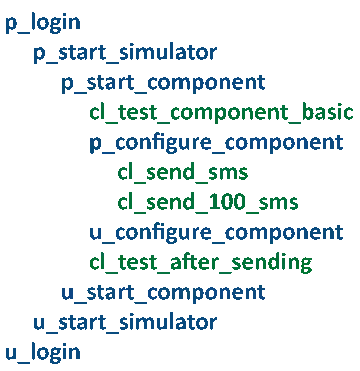
\includegraphics[scale=1]{ukazka_planu_testov}
    \caption{Ukážka plánu testov}
    \label{obrazok:ukazka_planu_testov}
  \end{center}
\end{figure}

Jednotlivé testy sa potom vykonávajú sekvenčne. Výhodou tohto prístupu 
je, že v~prípade, že sa zmena konfigurácie nepodarila, daný cluster 
môžeme preskočiť, a~tým ušetriť čas na dokončenie testovania. 
Test je úspešný, pokiaľ skončí s~nulovou návratovou hodnotou. 
V~opačnom prípade je test neúspešný.  
Ďalšou výhodou je znovupoužiteľnosť prerekvizít. 
Jednotlivé prerekvizity totiž môžeme kombinovať a~využiť ich tak pre 
potreby rôznych typov scenárov pre testy. 

Na obrázku \ref{obrazok:ukazka_planu_testov} je znázornený príklad štyroch 
clusterov, pričom platí, že clustre vyžadujú iné nastavenie systému. 
Z~obrázku je vidieť, že pre potreby clusterov \texttt{cl\_send\_sms}
a~\texttt{cl\_send\_100\_sms} je nutné vykonať prerekvizity \texttt{p\_connect}, 
\texttt{p\_start\_component}, \texttt{p\_start\_simulator} a~prerekvizitu 
\texttt{p\_configure\_component}. 
Zvyšným dvom clusterom stačia iba tri prerekvizity, a~to prerekvizita 
\texttt{p\_connect}, \texttt{p\_start\_simulator}
a~\texttt{p\_start\_component}. Cluster \texttt{cl\_test\_after\_sending} 
má rovnakú množinu prerekvizít ako cluster \texttt{cl\_test\_component\_basic}, 
a~spúšťa sa až za clusterom \texttt{cl\_send\_100\_sms}. 
Je preto nutné vrátiť zmeny systému, ktoré vykonala prerekvizita 
\texttt{p\_configure\_component} pomocou odrekvizity
\texttt{u\_configure\_component}. 
Takýmto spôsobom sa dosiahne, aby mal tento cluster rovnakú konfiguráciu 
systému ako cluster \texttt{cl\_test\_component\_basic}.
Po dokončení testovania všetkých clusterov ešte musíme spustiť zvyšné tri
odrekvizity, aby sa systém zanechal s~rovnakými nastaveniami, s~akými 
sa začínalo pri testovaní.

Pre zjednodušenie budú v~tomto dokumente všetky clustre zobrazené 
zelenou farbou.
Prerekvizity a~odrekvizity budú zobrazené modrou farbou. Takýmto spôsobom
si môžeme jednoducho znázorniť princíp plánovača testov, ktorý oddeľuje testy
slúžiace na testovanie funkčnosti systému, a~testy slúžiace na zmenu 
vlastností systému.

Jednotlivé prerekvizity na seba môžu, ale nemusia byť závislé, a~preto 
sa poradie spúšťania prerekvizít môže pre clustre meniť.
Príkladom závislosti môžu byť 2 prerekvizity, kde jedna prerekvizita 
zapína nejakú súčasť systému s~jeho defaultnými nastaveniami 
a~druhá prerekvizita tieto nastavenia mení. 
V~druhej prerekvizite môže byť preto nastavené, aby sa spustila, iba ak 
sa predtým úspešne splnila prerekvizita na zapnutie spomínanej časti 
systému. Plánovačka testov sa snaží plánovať jednotlivé clustre za seba 
tak, aby sa nemuseli nutne vykonať všetky prerekvizity a~odrekvizity pre 
každý cluster zvlášť. Znamená to, že ak majú dva clustre niektoré 
prerekvizity rovnaké, tak sa tieto clustre naplánujú tak, že sa rovnaké 
prerekvizity združia a~spúšťajú sa spravidla len raz. 
Táto vlastnosť je znázornená na obrázku 
\ref{obrazok:ukazka_zdruzovania_testov}. 
Ľavá časť obrázku ukazuje, ako by vyzeral plán, ak by plánovač testov
nedisponoval vlastnosťou združovania testov.

\begin{figure}[h]
  \begin{center}
    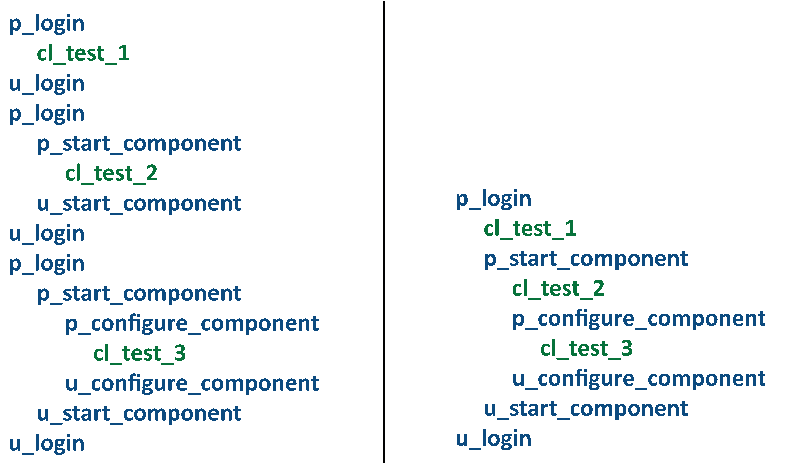
\includegraphics[scale=1]{ukazka_zdruzovania_testov}
    \caption{Ukážka vlastnosti združovania testov}
    \label{obrazok:ukazka_zdruzovania_testov}
  \end{center}
\end{figure}

V~regresnej sade sa bežne nachádzajú clustre, ktoré majú rovnakú množinu 
prerekvizít. Takéto clustre sa radia za seba, aby sa minimalizovalo
spúšťanie prerekvizít a~odrekvizít, ktoré majú spoločné. Neplatí teda 
pravidlo, že každý cluster má svoju vlastnú unikátnu prerekvizitu.



Medzi ďalšie výhody tohto plánovača testov patrí možnosť špecifikovania 
pravidiel, s~akými sa budú dané testy spúšťať. Je napríklad možné 
nastaviť clusteru zoznam clusterov, takzvaných preoptov, ktoré musia byť 
úspešne vykonané ešte predtým, ako sa vykoná samotný cluster. V~prípade, 
že sa aspoň jeden z~týchto preoptov nevykoná úspešne, cluster sa preskočí.
Výhoda tohto prístupu je v~tom, že ak zo sady testov, ktoré testujú 
podobnú funkcionalitu, neprejde najzákladnejší test, môžeme predpokladať, 
že všetky pokročilejšie testy by neprešli tiež, a~preto ich môžeme preskočiť.

Jednotlivé testy môžeme označovať vhodne zvoleným názvom nejakej 
funkcionality, pričom môžeme využiť vlastnosť plánovača, ktorý nám 
naplánuje len testy zvolené týmto názvom. Týmto spôsobom môžeme 
v~regresnej sade vytvárať isté logické celky, ktoré v~prípade potreby 
môžeme otestovať samostatne. Pre regresný beh je použitá funkcionalita 
\emph{all}, ktorá združuje všetky testy, ktoré nie sú explicitne označené 
funkcionalitou \emph{notall}. Obrázok \ref{obrazok:priklad_spustania_testov} 
znázorňuje príkaz pre spúšťanie regresných testov pomocou plánovača testov 
v~produkte MCO.

\begin{figure}[h]
\begin{lstlisting}
meszarosf@mco-v156#./Run_test.tcl -i cfg.ini -B TEST.REVIEW_23 -f all -tw
\end{lstlisting}
\caption{Príklad spúšťania regresných testov pomocou použitého plánovača}
\label{obrazok:priklad_spustania_testov}
\end{figure}

Za zmienku patrí aj možnosť označiť niektoré testy do kategórie 
známych chýb, označenej ako \emph{known bugs}. 
Testy z~tejto kategórie sú v~prípade zlyhania vylúčené zo zoznamu 
testov, ktoré zlyhali.
Typicky sa takto označujú testy, ktoré úspešne testujú nejakú 
funkcionalitu, ale vďaka nejakej nesúvisiacej chybe 
dopadajú neúspechom. Ďalej sa táto funkcionalita využíva napríklad pre 
testy, ktoré testujú nejakú časť systému, ktorá sa nestihla do danej 
vydanej verzie produktu opraviť. V~prípade, ak je test hotový, tak sa 
nechá v~regresnej sade, ale pre danú verziu sa označí do kategórie 
známych chýb, alebo anglicky known bugs.
Takýmto testom je možné explicitne uviesť rozsah verzie softvéru, 
v~ktorom je tento test chybný. Tieto testy aj spolu s~verziami softvéru, 
v~ktorom sa chyby prejavujú, sú uložené v~súbore \emph{KNOWN.BUGS}.
Príklad označenia testu, ktorý končí neúspechom vďaka nejakej 
nesúvisiacej chybe je znázornený na obrázku \ref{obrazok:known_bug}.
Tento test testuje chybu, ktorá sa objavila vo verzii produktu 2.3-05.01, 
avšak opravená bola až vo verzií 2.3-05.02. 

\begin{figure}[h]
\begin{lstlisting}[mathescape]
# MCRD0112570 (Problem with response to SMPP Bind operation)
cl_smpp_028                   >=2.3-05.01 $\sim$ >=2.3-05.02
\end{lstlisting}
\caption{Príklad testu ktorý končí neúspechom pre verziu softvéru 2.3-05.01.}
\label{obrazok:known_bug}
\end{figure}

Medzi poslednú vlastnosť, ktorú si spomenieme, je možnosť interaktívneho módu.
Interaktívny mód je vlastnosť, ktorá nám umožňuje pozastaviť beh 
testovania pred alebo za nejakým testom.
Umožňuje prípadne pozastaviť beh testovania, ak sa niektorý test 
ukončí neúspechom. Pozastavenie plánovača znamená, že je možné si 
v~špeciálnom režime spúšťať vlastné funkcie alebo celé testy.
Interaktívny mód umožňuje zmeniť beh testovania na základe špecifických 
požiadaviek testera, ktorý túto vlastnosť využíva.
Tento mód sa však v~regresných testoch nepoužíva, nakoľko sa narušuje 
vlastnosť nezávislosti testera na priebehu regresného testovania.

Spomínaný plánovač testov má ešte niekoľko vlastností, ktoré však nie sú
pre zameranie tejto bakalárskej práce dôležité. Tieto vlastnosti
v~kapitole nie sú uvedené pre ich rozsah. 

Každý test má svoj zdrojový kód v~spomínanom jazyku Tcl/Tk a~svoju 
vlastnú hlavičku, ktorá obsahuje informácie, potrebné pre identifikovanie 
testu a~jeho úspešné zaradenie do regresnej sady.
Zdrojové kódy testov sú logicky rozdelené a~umiestnené v~súboroch 
začínajúcich predponou \emph{CL-} a~s~príponou \emph{.tcl}, 
napríklad \emph{CL-SMPP.tcl} alebo \emph{CL-GSM.tcl}.
Hlavičky testov môžu byť taktiež logicky delené na niekoľko celkov 
a~začínajú predponou \emph{TEST.}, napríklad \emph{TEST.ALL} alebo 
\emph{TEST.REVIEW\_23}.
Takýmto spôsobom sú napríklad delené testy, ktoré prešli kontrolou,
a~sú úspešne zaradené do regresnej sady (súbor \emph{TEST.ALL}) a~testy, 
ktoré sú do regresnej sady zaradené, ale zatiaľ neboli nikým 
skontrolované (súbor \emph{TEST.REVIEW\_23}).

Hlavička každého testu je štandardizovaná a~obsahuje nasledovné informácie:
\begin{itemize}
\item \textbf{Name} -- názov testu
\item \textbf{Author} -- autor testu
\item \textbf{Description} -- stručný popis toho, čo daný test vykonáva
\item \textbf{Function} -- názov funkcie v~jazyku Tcl/Tk, ktorá sa daným 
testom spustí. Každý test je tvorený jednou funkciou, ktorá je typicky 
rovnaká ako názov testu. Ako nepovinný parameter je možné špecifikovať 
argumenty funkcie. Príkladom môže byť cluster s~názvom 
\texttt{cl\_send\_sms} ktorý používa ako argument počet sms správ ktoré 
má poslať, s~defaultnou hodnotou 100 sms správ 
má označenú túto položku ako \texttt{cl\_send\_sms 10000}. 
V~regresnej sade potom existuje test \texttt{cl\_send\_sms\_long\_running}, 
s~položkou Function označenou ako \texttt{cl\_send\_sms 10000}, ktorý 
posiela takýchto správ stonásobne viac.
\item \textbf{Pre} -- množina všetkých prerekvizít, ktoré musia byť 
v~čase spustenia daného testu úspešne aktivované. 
Princíp plánovača je ten, že prerekvizity sú určené na zmenu stavu 
testovacieho prostredia. Množina prerekvizít uvedených v~tejto položke 
teda predstavuje prerekvizity, ktoré je nutné úspešne spustiť, aby sme 
testovacie prostredie dostali do stavu, v~ktorom bude možné spustiť 
aktuálny test.
\item \textbf{Preopt} -- množina všetkých clusterov, ktoré musia byť 
úspešne spustené v~čase, keď sa púšťa aktuálny test. 
Ak aspoň jeden cluster z~tejto množiny dopadol neúspechom, aktuálny 
cluster sa preskočí. Táto položka je určená iba pre clustre.
\item \textbf{Restore} -- názov prerekvizity, ktorá patrí je určená pre 
nastavenie testovacieho prostredia pre potreby testu. 
Táto položka je určená iba pre odrekvizity.
\item \textbf{Undo} -- názov odrekvizity, ktorá je určená pre obnovu 
testovacieho prostredia. Táto položka je určená iba pre prerekvizity. 
\item \textbf{Functionalities} -- množina všetkých názvov funkcionalít, 
ktorými je možné daný test spustiť. 
Táto položka umožňuje logicky rozdeliť všetky testy do podmnožín, 
ktoré je možné spúšťať samostatne. 
Plánovač umožňuje pomocou prepínača \texttt{-f} určiť, ktoré 
funkcionality sa pri testovaní spustia.
Pred naplánovaním testov sa nájdu sa všetky testy, ktoré sú týmito 
funkcionalitami označené, a~tieto testy sa naplánujú. 
Štandardná hodnota pre všetky clustre je hodnota \texttt{all}, a~pre 
všetky prerekvizity a~odrekvizity je to hodnota \texttt{notall}.
Typickým príkladom použitia je nastavenie testov, ktoré sa v~nočných 
regresiách bežne nepúšťajú, nakoľko je ich beh príliš časovo náročný, 
na hodnotu \texttt{long\_running}.
V~plánovači je potom možné spustiť funkcionalitu \texttt{all} bez testov, 
ktoré sú označené funkcionalitou \texttt{long\_running}.
\item \textbf{Sets} -- umožňuje ďalší spôsob logického rozdeľovania testov 
na podmnožiny, podobne ako položka \texttt{Functionalities}.
\item \textbf{Versions} -- dolné a~prípadne aj horné ohraničenie hodnoty 
verzie softvéru, na ktorej je daný test možné pustiť
(Napríklad test určený pre softvér od verzie 2.3-0.0 vrátane, 
až do verzie 2.3-04.06 môžeme označiť ako: \textgreater= 2.3-00.00 
$\sim$ \textgreater= 2.3-04.06).
\item \textbf{CR} -- popisok slúžiaci na označenie čísla ticketu, alebo 
čísla zmeny požiadavkov systému\footnote{angl. change request}, ktoré sú 
do systému implementované na vyžiadanie zákazníka. 
Pomocou prepínača \texttt{-cr} v~plánovači je možné spustiť všetky testy, 
ktoré majú dané označenie v~tejto položke.
\item \textbf{CRS} -- informačný popisok slúžiaci na označenie konkrétnej 
časti naimplementovanej zmeny systému. 
\end{itemize}

Príklad hlavičky testu zo súboru \emph{TEST.REVIEW\_23} je zobrazený na 
obrázku \ref{obrazok:hlavicka_testu}.

\begin{figure}[h]
\begin{lstlisting}
Cluster
Name: cl_smpp_truncate_025
Author: Filip Meszaros
Description: Priklad hlavicky testu zo suboru TEST.REVIEW_23
Function: cl_smpp_truncate_025
Pre: p_mobiles p_sol_default p_dc_default p_gbg_default p_sol_sf p_smpp_truncate
Preopt: cl_smpp_truncate_001
Restore:
Undo:
Functionalities: smpp truncate licensed gsm
Sets:
Versions: >= 2.3-05.01
CR: MCRE0112412 CR00025702 MCRE0112535
CRS:
\end{lstlisting}
\caption{Príklad hlavičky testu}
\label{obrazok:hlavicka_testu}
\end{figure}


Táto sekcia obsahovala zhrnutie toho, akým princípom funguje plánovač 
testov, vytvorený firmou Acision. Niektoré vlastnosti a~funkcionalita 
plánovača v~tejto kapitole nie sú popísané, nakoľko nie sú predmetom 
tejto bakalárskej práce. Na záver si ešte uvedieme zoznam výhod a~nevýhod 
použitia tohto nástroja.

\noindent \textbf{Výhody}:
\begin{itemize}
\item jednoduché zaradenie nového testu do regresnej sady
\item možná znovupoužiteľnosť prerekvizít
\item združovanie prerekvizít
\item preskakovanie testov o~ktorých vieme, že by skončili neúspechom
\item možné označovanie testov do kategórie známych chýb (súbor KNOWN.BUGS)
\item interaktívny mód pre testovanie
\item označovanie testov do logických celkov a~ich spúšťanie
\item oddelený kód pre zmenu konfigurácie a~pre samotné testy
\item veľká možnosť zmien chovania pomocou prepínačov
\end{itemize} 

\noindent \textbf{Nevýhody}:
\begin{itemize}
\item náhodný neúspech nejakej prerekvizity môže znamenať vynechanie 
väčšiny testov v~regresnom testovaní
\item jeden chybne pridaný test môže znefunkčniť plánovač
\item jednotlivé testy sa v~prípade chyby systému nemusia úspešne z~tejto 
chyby zotaviť, a~môžu spustiť lavínu chýb, ktoré by inak nenastali 
\item v~prípade, že sa konfiguračné zmeny v~odrekvizitách úspešne neobnovia, 
dochádza k~neodpovedajúcim výsledkom z~testovania
\item plánovanie testov je relatívne pomalé
\item prehľad v~testoch a~ich údržba je náročná
\end{itemize}



%
% Kapitola 3
%
\chapter{Návrh riešenia}
\label{kapitola:navrh_riesenia}
Táto kapitola sa zaoberá základným návrhom implementácie rozšírenia 
plánovača testov pre podporu distribuovania testov na viaceré systémy. 
Kapitola popisuje rôzne možnosti distribuovania testov, ich vzájomné 
porovnanie a~taktiež výhody a~nevýhody jednotlivých prístupov. 
V~kapitole si popíšeme návrh spúšťania testov a~prístup k~centralizovanej 
správe plánovača testov. Ďalej si popíšeme návrh riešenia komunikácie 
medzi jednotlivými regresnými behmi, vykonávaných na samostatných 
testovacích strojoch, na spôsob čakania na dokončenie testovania. 
V~kapitole je taktiež popísaný návrh zbierania výsledkov a~ich interpretácia.
Posledná časť kapitoly poukazuje na nové typy problémov, ktoré vznikli pri
vytváraní rozšírenia plánovača testov, a~navrhuje možnosti ich riešenia.


\section{Možnosti distribuovania testov}
\label{sekcia:moznosti_distribuovania}
Pri návrhu distribuovania testov som vychádzal z~informácií o~počte 
testov a~prerekvizít produktov, ktoré daný plánovač testov používajú. 
Informácie som čerpal z~dvoch najväčších produktov (MCO a~SMSCv5), 
ktoré tento plánovač testov každodenne používajú. 
Pri každom regresnom behu sa zbierajú štatistiky o~tom,
koľko testov bolo spustených, a~ako dlho každý test trval. 
V~tabuľkách \ref{tabulka:testy_mco} a~\ref{tabulka:testy_smsc} sú 
zobrazené informácie o~testoch z~týchto dvoch najväčších produktov.

\begin{table}
  \begin{center}
    \begin{tabular}{| c | r | r | r | r | r | r |}
    \hline
    typ testu & počet testov & min. čas [s] & max. čas[s] & 
    priem. čas [s] & modus & medián \\ \hline
    cluster      & 1791 & 1 & 931 & 18,47 & 8  & 7 \\ \hline
    prerekvizita & 323  & 1 & 82  & 19,54 & 18 & 1 \\ \hline
    odrekvizita  & 323  & 1 & 63  & 19,56 & 18 & 7 \\
    \hline
    \end{tabular}
    \caption{Prehľad testov dostupných pre najnovšiu verziu produktu MCO 
             a~štatistiky o~dĺžke trvania testov v~sekundách}
    \label{tabulka:testy_mco}
  \end{center}
\end{table}

\begin{table}
  \begin{center}
    \begin{tabular}{| c | r | r | r | r | r | r |}
    \hline
    typ testu & počet testov & min. čas [s] & max. čas [s] & 
    priem. čas [s] & modus & medián \\ \hline
    cluster      & 1810 & 1 & 1963 & 26,19 & 12 & 3 \\ \hline
    prerekvizita & 247  & 1 & 120  & 9,82  & 6  & 1 \\ \hline
    odrekvizita  & 247  & 1 & 78   & 6,96  & 5  & 1 \\
    \hline
    \end{tabular}
    \caption{Prehľad testov dostupných pre najnovšiu verziu produktu SMSCv5 
             a~štatistiky o~dĺžke trvania testov v~sekundách}
    \label{tabulka:testy_smsc}
  \end{center}
\end{table}

Z~tabuliek je vidieť, že produkt MCO má priemerné časy clusterov, 
prerekvizít a~odrekvizít veľmi podobné. V~produkte SMSCv5 je priemerný 
čas vykonávania clusterov niekoľkonásobne vyšší, ako priemerný čas 
vykonávania prerekvizít alebo odrekvizít.
Tieto tabuľky však ukazujú celkový počet všetkých testov. 
Niektoré testy sú však z~regresnej sady vynechané.
Navyše z~tabuliek nie je jasné, koľko prerekvizít sa skutočne naplánuje 
pre jeden beh regresií. Z~konceptu plánovača totiž vyplýva, že niektoré 
prerekvizity je nutné spúšťať viacnásobne.
Je to preto, lebo každý cluster môže mať inú množinu prerekvizít
a~všetky tieto kombinácie možných prerekvizít pre každý cluster
je potrebné naplánovať.

\begin{table}
  \begin{center}
    \begin{tabular}{| c | r | r |}
    \hline
    typ testu    & počet testov pre produkt MCO & 
    počet testov pre produkt SMSCv5 \\ \hline
    cluster      & 1710 & 1716 \\ \hline
    prerekvizita & 707  & 661  \\ \hline
    odrekvizita  & 707  & 661 \\
    \hline
    \end{tabular}
    \caption{Prehľad počtu naplánovaných testov pri regresnom testovaní 
             v~produktoch MCO a~SMSCv5}
    \label{tabulka:pocet_naplanovanych_testov}
  \end{center}
\end{table}

Tabuľka \ref{tabulka:pocet_naplanovanych_testov} zobrazuje počet 
clusterov a~prerekvizít, ktoré sa plánujú pri každodennom spúšťaní 
nočných regresií pomocou funkcionality \texttt{all} a~v~prípade produktu 
SMSCv5 aj pomocou funkcionality \texttt{2nd}. Z~tabuľky vyplýva, že 
približne 5\% testov sa z~nočných regresií vynecháva. 
Túto množinu tvoria napríklad testy, ktoré nie sú plne automatické, 
a~vyžadujú tak interakciu s~používateľom, alebo testy, o~ktorých sa vie, 
že je nevhodné ich spúšťať spolu s~veľkou množinou testov, 
nakoľko môžu negatívne ovplyvniť výsledky týchto testov.
Zároveň z~obrázku vyplýva to, že sa spustí viac ako dvojnásobok 
prerekvizít, ako existuje v~testovacej sade. Každá prerekvizita sa teda 
spustí v~priemere viac ako dvakrát. Vo svetle týchto informácií je teda 
vhodné zameriavať sa pri rozdeľovaní testov na clustre.

V~nasledujúcej časti sa pozrieme na navrhnuté možnosti distribuovania 
testov, ich výhody a~nevýhody. Treba podotknúť, že plánovač testov si 
uchováva čas behu každého naposledy spusteného testu.
Táto štatistika sa môže využiť pri distribuovaní testov, aby sme vedeli 
rovnomerne rozložiť záťaž pre každý systém.
\subsubsection*{Distribúcia clusterov na základe dĺžky behu clusterov}
Tento princíp distribúcie by spočíval v~rozdeľovaní clusterov do \textit{n} 
podmnožín na základe súčtu časov trvaní všetkých clusterov v~danej podmnožine. 
Každý cluster by bol zaradený do jednej podmnožiny, pričom by platilo,
že každá podmnožina by sa spúšťala na samostatnom testovacom systéme. 
Pri rozdeľovaní testov na podmnožiny by sa bral zreteľ na distribuovanie 
záťaže.
\\
\\
\noindent \textbf{Výhody}:
\begin{itemize}
\item jednoduché na implementáciu
\end{itemize} 

\noindent \textbf{Nevýhody}:
\begin{itemize}
\item odhadovaný čas každej podmnožiny clusterov by nereflektoval stav 
po naplánovaní, pretože by neobsahoval čas potrebný pre spustenie 
prerekvizít a~odrekvizít
\item neefektívne združovanie prerekvizít
\item nerovnomerné rozloženie záťaže
\end{itemize}

\subsubsection*{Distribúcia clusterov na základe spoločných prerekvizít}
Distribúcia na základe spoločných prerekvizít využíva fakt, že 
v~regresnej sade existujú testy, ktoré majú rovnakú množinu prerekvizít.
Celú regresnú sadu môžeme týmto spôsobom rozdeliť na \emph{n} podmnožín, 
pričom by platilo, že všetky clustre v~jednej takejto množine by mali
rovnakú množinu prerekvizít. Pri distribúcií testov na \emph{m} častí, 
ktoré by sa spúšťali samostatne, by sa do jednotlivých \emph{m} častí
priraďovali vždy celé podmnožiny \emph{n}. 
Obrázok \ref{obrazok:podmnoziny_testov} ilustruje delenie clusterov do 
štyroch \emph{n} podmnožín. Pri distribúcií testov by sa potom každá 
takáto podmnožina brala ako celok a~distribuovali by sme tak 
jednotlivé podmnožiny.
Obrovskou výhodou tohto prístupu je to, že vo výsledku by sme ušetrili 
spúšťanie niekoľkých prerekvizít, nakoľko by sa využila vlastnosť 
plánovača, a~tou je združovanie testov. Príkladom výsledku môže byť 
napríklad distribuovanie testov na 2 systémy, pričom prvý systém by 
spúšťal clustre z~podmnožiny 1 a~4 (clustre \texttt{cl\_subset1\_test1}, 
\texttt{cl\_subset1\_test2} a~\texttt{cl\_subset4\_test1})
a~druhý systém by spúšťal clustre z~podmnožiny 2 a~3 
(clustre \texttt{cl\_subset2\_test1}, \texttt{cl\_subset2\_test2}, 
\texttt{cl\_subset2\_test3}, \texttt{cl\_subset3\_test1} 
a~cluster \texttt{cl\_subset3\_test2}).

\begin{figure}[h]
  \begin{center}
    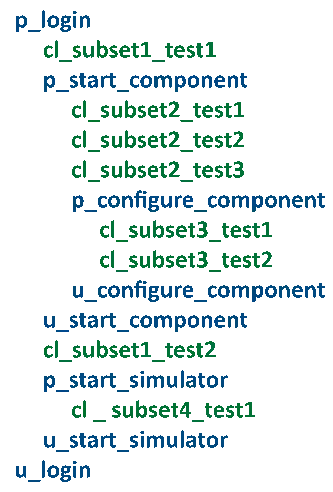
\includegraphics[scale=1]{ukazka_podmnozin}
    \caption{Príklad rozdeľovania clusterov na podmnožiny na 
             základe spoločných prerekvizít}
    \label{obrazok:podmnoziny_testov}
  \end{center}
\end{figure}


\noindent \textbf{Nevýhody}:
\begin{itemize}
\item nedokonalé združovanie prerekvizít 
\item odhadovaný čas každej podmnožiny clusterov by nereflektoval stav 
po naplánovaní, pretože by neobsahoval čas potrebný pre spustenie 
prerekvizít a~odrekvizít
\end{itemize}

\subsubsection*{Distribúcia clusterov na základe častí plánu}
Idea tohoto prístupu spočíva v~tom, že by sa všetky testy naplánovali 
ako obvykle, a~po naplánovaní by sa celý plán rozdelil na \emph{m} častí. 
Plánovač by spočítal odhadované časy jednotlivých častí a~snažil by 
sa tieto časti rozdeliť rovnomerne. Po rozdelení by sa do každej časti 
museli pridať prerekvizity a~odrekvizity, o~ktoré by sme daným 
delením prišli. 
Princíp rozdelenia plánu na 3 časti je znázornený na obrázku 
\ref{obrazok:distribucia_na_casti}.

\begin{figure}[h]
  \begin{center}
    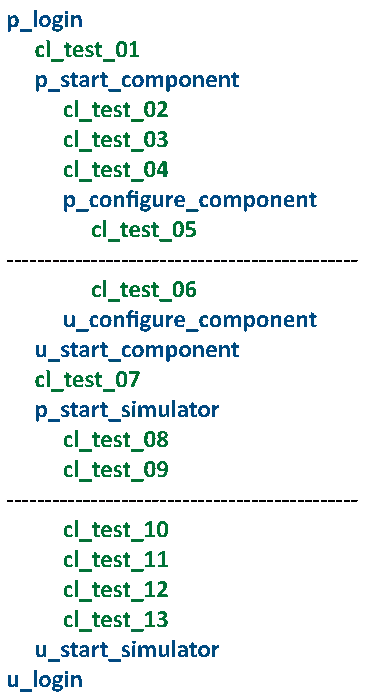
\includegraphics[scale=1]{delenie_planu_na_casti}
    \caption{Príklad rozdeľovania clusterov na základe častí plánu}
    \label{obrazok:distribucia_na_casti}
  \end{center}
\end{figure}

Po rozdelení je dôležité, aby sme každej časti pridali prerekvizity 
a~odrekvizity, o~ktoré sme prišli pri delení. Ak sa tieto testy pridajú 
do plánu, celý plán pre 3 systémy by vyzeral tak, ako je znázornené na 
obrázku \ref{obrazok:distribucia_casti_po_preplanovani}.
Z~obrázku vyplýva, že pre vysoký počet testov by bol tento prístup 
najvhodnejší. Problémom tohto prístupu je však to, že požiadavkom na 
funkcionalitu plánovača bolo to, aby sa princíp plánovania testov nezmenil. 
Znamená to, že by sa museli rešpektovať hlavičky testov napríklad na 
položku \emph{Preopt}, čo znamená, že každému clusteru môžeme nastaviť 
množinu clusterov, ktoré musia byť úspešne otestované ešte predtým, 
ako sa spustí test aktuálneho clusteru.
Príkladom tohto problému je prípad, kedy by cluster \emph{cl\_test\_13} 
mal nastavený \textit{Preopt} na cluster \emph{cl\_test\_01} 
a~\emph{cl\_test\_06}.
V~praxi by to znamenalo, že celá tretia časť rozdeleného plánu by sa 
musela preplánovať a~spomínané clustre by sa do nej museli pridať. 
Ďalšou nevýhodou je to, že tento prístup by vyžadoval väčší zásah do 
funkčnosti plánovača testov, nakoľko by sa celá logika plánovača musela upraviť.
V~prípade, že by ale neexistovala požiadavka na zachovanie funkčnosti, 
tento prístup by bol najvhodnejší. Týmto problémom, spôsobeným zachovaním 
funkcionality plánovača, trpia aj predošlé 2 spôsoby distribúcie testov. 
Pre povahu testov v~regresnej sade by však najviac na toto doplácal 
práve tento princíp distribuovania testov.  

\noindent \textbf{Výhody}:
\begin{itemize}
\item efektívne združovanie prerekvizít
\item veľmi presné rozloženie záťaže 
(v~prípade nezachovania požiadavkov na funkcionalitu)
\item presný odhad trvania testovania 
(v~prípade nezachovania požiadavkov na funkcionalitu)
\end{itemize} 

\noindent \textbf{Nevýhody}:
\begin{itemize}
\item náročné na implementáciu, pretože by sa musela zmenila logika plánovača
\end{itemize}

\begin{figure}[h]
  \begin{center}
    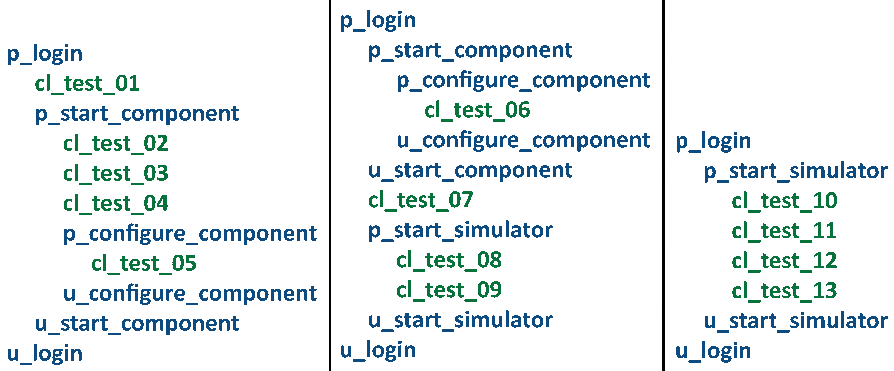
\includegraphics[scale=1]{casti_po_preplanovani}
    \caption{Príklad rozdeľovania clusterov na základe častí plánu
             - po preplánovaní}
    \label{obrazok:distribucia_casti_po_preplanovani}
  \end{center}
\end{figure}

\section{Centralizovaná správa plánovača}
\label{sekcia:centralizovana_sprava}
Jedným z~hlavných vlastností, spomínaných v~dokumente 
\cite{Parallel_approach},  ktoré by mal mať nástroj pre distribúciu 
testov, je vlastnosť  centralizovanej správy všetkých testov. 
Pri návrhu rozšírenia plánovača  sa táto vlastnosť brala do~úvahy. 
Rozšírenie je navrhnuté tak, aby bolo  z~jedného stroja možné spustiť 
rozšírený plánovač, ktorý by rozdelil množinu 
testov na \emph{m} podmnožín, v~závislosti na počtu strojov, na ktorých 
chceme regresné testy spustiť. Jednotlivé podmnožiny testov sa 
potom predajú novým inštanciám plánovačom testov, ktoré by tieto testy 
preplánovali a~začali by ich vykonávať. 
Tieto nové inštancie plánovačov sú spustené ako podprocesy hlavného procesu, 
ktorým je rozšírený plánovač testov.
Plánovač testov je navrhnutý tak, aby dokázal rozdistribuovať testy na 
teoreticky nekonečný počet neprázdnych podmnožín.
V~prípade, že je počet testovacích systémov väčší ako počet clusterov, 
niektoré testovacie systémy sa nevyužijú.
Centralizovaná správa plánovača umožňuje zobraziť rozdelený plán 
testovania pre každý testovací systém zvlášť. Zároveň umožňuje vypísať 
odhadované časy testovania pre každý systém zvlášť a~umožňuje porovnanie 
efektivity distribuovania testov voči stavu, kedy by testy neboli 
distribuované, a~spúšťali by sa iba na jednom systéme. 

Pri navrhovaní riešenia pre centralizovanú správu testov bolo nutné 
vymyslieť, akou formou sa budú spúšťať jednotlivé inštancie plánovača pre 
distribuované systémy. Plánovač testov totiž potrebuje konfiguračný súbor,
zadávaný parametrom \textbf{-i}, ktorý je uvedený napríklad na obrázku 
\ref{obrazok:priklad_spustania_testov}.
Tento konfiguračný súbor obsahuje informácie ako IP adresa systému, na ktorom sa 
budú spúšťať testy, číslo verzie softvéru, názov 
produktu, atď. Príklad takéhoto konfiguračného súboru je znázornený na 
obrázku \ref{obrazok:priklad_konfig_suboru}.
Rozšírenie plánovača pre distribuované systémy však potrebuje informácií 
obsiahnutých v~konfiguračnom súbore viac.
Pre každý distribuovaný systém potrebuje napríklad jednu IP adresu 
obsiahnutú v~položke \textit{Host}.
Jedným riešením by bolo dať všetky informácie pre každý distribuovaný 
systém do jedného konfiguračného súboru.
V~tomto jednom súbore by sa potom dalo napríklad nastavovať, na koľkých 
testovacích systémoch sa regresné testy spustia.
Pre toto riešenie by však bolo treba upraviť parser, ktorý informácie 
z~týchto konfiguračných súborov vyhodnocuje.
Mnou navrhnuté riešenie teda počíta s~jedným konfiguračným súborom pre 
každý testovací systém.
Pri spúšťaní regresných testov na troch systémoch je preto potrebné 
mať pripravené 3 konfiguračné súbory, každý pre jeden testovací systém. 

\begin{figure}[h]
\begin{lstlisting}
Product: MCO
Username: root
Host: 10.10.10.206
Outerhost: 10.10.110.206
Version: 2.3-05.04
\end{lstlisting}
\caption{Príklad konfiguračného súboru pre produkt MCO}
\label{obrazok:priklad_konfig_suboru}
\end{figure}

Nová funkcionalita, ktorá bola pridaná do rozšíreného plánovača, je 
možnosť sledovať aktuálny stav testovania formou progress baru. 
Táto funkcionalita v~starej verzii plánovača testov chýbala a~bolo 
preto ťažké sledovať aktuálny stav testovania. 
V~rozšírenej verzií plánovača sa zobrazuje aktuálny stav testovania pre 
každý systém zvlášť, ako aj celkový stav všetkých testov.

\section{Komunikácia medzi jednotlivými plánovačmi testov}
\label{sekcia:komunikacia}
V~distribuovaných systémoch nie je spoločná pamäť, a~preto je forma 
komunikácie založená na princípe zasielania správ.
Princíp komunikácie je taký, že hlavný proces, ktorý spustí \emph{m} 
plánovačov testov vo forme podprocesov, čaká na ukončenie
všetkých týchto podprocesov. Ukončenie podprocesu znamená, že ak 
nenastala žiadna systémová chyba, tak je testovanie jednej podmnožiny 
testov dokončené. Ak by náhodou nastala nejaká kritická chyba, 
podproces by sa mohol ukončiť, a~my by sme mohli prísť o~výsledky 
z~tejto podmnožiny regresných testov. Z~tohto dôvodu by sa výsledky 
z~testovania mali posielať ihneď, ako ich máme k~dispozícií,
a~nemalo by sa čakať na dokončenie testovania danej podmnožiny 
regresných testov. Každý podproces teda asynchrónne zasiela údaje 
o~výsledkoch aktuálneho testu hlavnému procesu, ktorý si tieto výsledky 
uchováva. Tento prístup má výhodu, že sa výsledky testovania uchovávajú 
na dvoch miestach, a~v~prípade zlyhania systému, či už hlavného procesu 
alebo podprocesov, by sme sa k~daným výsledkom vedeli dopracovať. 


\section{Interpretácia výsledkov}
\label{sekcia:interpretacia_vysledkov}
Medzi jednu z~najdôležitejších vlastností, ktoré musí každý testovací 
nástroj mať, je vlastnosť zobrazovania výsledkov z~testovania.
Pri návrhu rozšírenia plánovača testov bolo nutné riešiť situáciu, 
ako zobraziť výsledky z~každého testovacieho systému jednotlivo,
a~takisto aj súhrn celkových výsledkov. 

Rozšírenie plánovača testov disponuje niekoľkými výsledkami, ktorými 
môže každý test skončiť. Jednotlivé výsledky platia len v~prípade, že 
sa daný test spúšťal na všetkých testovacích systémoch len raz. 
Sú to výsledky:
\begin{itemize}
\item \textbf{passed} -- test, ktorý sa skončil úspechom 
(návratová hodnota je rovná nule).
\item \textbf{failed} -- test, ktorý sa ukončil neúspechom 
(nenulová návratová hodnota).
\item \textbf{skipped} -- test, ktorý sa vďaka neúspechu nejakého predošlého 
testu vynechal, nakoľko by jeho spustenie skončilo neúspechom.
\item \textbf{passed on second attempt} -- cluster, ktorý sa vďaka 
prepínaču plánovača \textbf{-tw} spustil po neúspechu znova, pričom na 
druhýkrát skončil úspechom. 
Test označený týmto výsledkom je zároveň označený výsledkom \textbf{passed}
\item \textbf{known bug - failed} -- cluster, ktorý je pre aktuálnu 
verziu softvéru označený ako \textbf{known bug}, ktorý skončil úspechom. 
Cluster označený týmto výsledkom, nie je označený výsledkom \textbf{failed}.
\item \textbf{known bug - passed} -- cluster, ktorý je pre aktuálnu 
verziu softvéru označený ako \textbf{known bug}, ktorý skončil neúspechom.
Cluster označený týmto výsledkom je zároveň označený aj výsledkom 
\textbf{passed}.
\end{itemize} 

V~prípade, že sa nejaký test spúšťal na viacerých systémoch, bolo nutné 
riešiť stav, v~ktorom sa test mohol ocitnúť. Problémom je situácia, 
kedy nejaký test, ktorý sa spúšťal na viacerých systémoch, skončil na 
týchto rozdielnych systémoch s rôznymi výsledkami.
Pre riešenie tejto situácie bol zavedený stav \textbf{unclear}. 
Ak test skončí s~rôznymi výsledkami, jeho finálny výsledok sa určí podľa 
prevodovej tabuľky \ref{tabulka:vysledky_testu_prevod}.
Stavy \emph{passed on second attempt}, \emph{known bug - failed}
a~\emph{known bug - passed} nie sú zaznačené z~dôvodu, že tieto špeciálne 
stavy sa mapujú na stavy \emph{failed} a~\emph{failed}.

Spomínané stavy výsledkov testov platia pre celkové výsledky zo všetkých 
testovacích systémov. Rozšírený plánovač testov navyše umožňuje zobraziť 
výsledky všetkých testov pre každý testovací systém jednotlivo. 
Výsledok každého testu sa zobrazuje v~rovnakom poradí, ako sa testy spúšťali.
Každý zobrazovaní výsledkov z~každého testovacieho systému majú však 
testy pre jednoduchosť len stavy \emph{passed}, \emph{failed} 
a~\emph{skipped}. 

\begin{table}
  \begin{center}
    \begin{tabular}{| c | c | c |}
    \hline
    výsledok 1  & výsledok 2 & konečný výsledok \\ \hline
    passed      & passed     & passed  \\ \hline
    failed      & failed     & failed  \\ \hline
    skipped     & skipped    & skipped \\ \hline
    passed      & skipped    & passed  \\ \hline
    failed      & skipped    & failed  \\ \hline
    passed      & failed     & unclear \\ \hline
    unclear     &      *     & unclear \\ \hline
    \end{tabular}
    \caption{Mapovanie rozdielnych výsledkov testu na konečný výsledok}
    \label{tabulka:vysledky_testu_prevod}
  \end{center}
\end{table}



\section{Riešenie nových typov problémov}
\label{sekcia:riesenie_novych_problemov}
Pri vytváraní rozšírenia plánovača je potrebné myslieť na nové problémy, 
ktoré sa objavili až pri riešení distribúcie testov. 
Jedným z~problémov je zobrazovanie výsledkov testov, spomínané 
v~predchádzajúcej kapitole. Pre riešenie tohto problému bol zavedený 
výsledok testu\emph{unclear}.

\subsection*{Nezávislosť medzi testami}
Ďalším z~problémov, ktorého riešenie bolo treba navrhnúť, bol problém, 
ktorý porušoval vlastnosť nezávislosti medzi testami a~vlastnosť 
integrity testovacej sady, popísaných v~dokumente \cite{Kapfhammer}.
Jednalo sa o~problém, že niektoré testy používali pevne stanovený 
sieťový port, ktorý slúžil napríklad pre komunikáciu so simulátorom, 
alebo pre napojenie sa na nejakú časť testovaného systému, atď.
Problémom tohto pevného portu bola distribúcia testov, 
ktoré používali rovnaký port. V~prípade, že sa takéto testy spúšťali naraz, 
dochádzalo k~obsadeniu portu prvým testom, pričom druhý test 
už k~portu nemal prístup, a~tak končil neúspechom.

Riešením tohto problému je parameter port offset \textbf{-po}. 
Každý test, ktorý používal pevne stanovenú hodnotu portu sa musel 
upraviť tak, aby sa ako port použila táto pevná hodnota, pripočítaná 
o~hodnotu zadanú parametrom \textbf{-po}.
Jednotlivé podprocesy plánovača testov sa spúšťajú s~parametrom 
\textbf{-po}, ktorý sa navyšuje práve o~hodnotu \textbf{-po} 
s~každým podprocesom. V~praxi to znamená, že ak nastavíme hodnotu 
offsetu na 1000, tak sa prvý podproces spustí s~parametrom
\textbf{-po 1000}, druhý podproces sa spustí s~parametrom \textbf{-po 2000}, 
tretí s~\textbf{-po 3000} atď. V~teste sa potom používa štandardné 
číslo portu, ktorý sa využíval v~teste pred úpravou, s~pridanou hodnotou 
port offsetu. Týmto spôsobom sa zabraňuje problému, že niektoré testy 
pristupovali k~rovnakému portu súčasne. Implicitnou hodnotou parametru 
\textbf{-po}, ktorá sa používa napríklad pri spustení plánovača testov
bez potreby distribúcie testov je hodnota 0. 

\subsection*{Systém logovania}
Ďalším novým problémom sa stalo aj spravovanie logovacích súborov. 
Plánovač testov totiž pri vykonávaní testov zapisuje informácie 
o~aktuálne prevádzaných testoch do viacerých logovacích súborov.
Pri distribuovaní testov sa však spúšťajú viaceré podprocesy plánovača 
testov, pričom každý podproces si tieto súbory vytvára zvlášť. 
V~rámci centrálnej správy bolo nutné navrhnúť prístup, akým sa budú
logovať testy z~viacerých strojov na jedno centrálne miesto.
Pre riešenie tohto problému bolo možné implementovať 2 možné spôsoby:
\begin{itemize}
\item \textbf{Zapisovanie údajov do logov po každom teste} -- 
týmto spôsobom by sa do logovacích súborov, vytváraných hlavným procesom,
postupne zapisovali informácie, vždy po aktuálne dokončenom teste, 
nezávisle na testovacom systéme. Tento prístup je však nevyhovujúci, 
lebo by podprocesy museli posielať logovacie informácie hlavnému procesu, 
čo je náročné na zdroje. Ďalšou nevýhodou je to, že by sa poradie 
jednotlivých testov z~testovacích systémov pomiešalo.
\item \textbf{Parsovanie údajov do logov po dokončení testovania} -- 
toto riešenie spočíva v~tom, že sa najprv počká na dokončenie testovania. 
V~momente, ak je testovanie ukončené, môžeme počítať so situáciou,
že každý podproces plánovačky testov si vytvoril vlastné logovacie súbory, 
v~ktorých je zachované poradie testov. Ak máme tieto súbory k~dispozícií, 
môžeme si z~nich vytiahnuť potrebné informácie a~skopírovať ich do 
logovacích súborov, vytvorených rozšíreným plánovačom testov. 
Toto riešenie má výhodu, že je menej náročné na zdroje, a~zároveň,
že sa v~logoch dodržiava poradie testov, vykonávaných pre každý systém zvlášť. 
Pri implementácií rozšírenia plánovača testov sa využíva práve toto riešenie.
\end{itemize} 

\subsection*{Neželané distribuovanie testov}
V~regresnej sade existujú množiny testov, ktoré chceme spúšťať vždy ako celok.
Príkladom takejto množiny testov je funkcionalita \textbf{env}, ktorá
slúži na nainštalovanie produktu MCO. Táto funkcionalita obsahuje 5 clusterov,
ktoré tvoria jeden funkčný celok slúžiaci na inštaláciu produktu.
Táto funkcionalita obsahuje clustre, ktoré v~prípade produktu MCO:
\begin{enumerate}
\item vymažú zo systému produkt MCO
\item stiahnu verziu produktu MCO zadanú v~konfiguračnom súbore
\item nainštalujú stiahnutú verziu produktu
\item nakonfigurujú systém
\item nainštalujú externé súčasti systému
\end{enumerate} 

V~prípade regresných testov sa pred samotným testovaním vždy vykoná táto 
funkcionalita, aby sa zaistilo, že je systém nainštalovaný nanovo.
Pri využívaní viacerých systémov pre distribúciu testov je nutné na každom
tomto systéme preinštalovať testovaný produkt. 
Pre tento účel bol naimplementovaný parameter 
\textbf{-wd}\footnote{skratka pre angl. without distribution}, 
ktorý zapríčiní, že testy sa nebudú distribuovať, ale po naplánovaní 
sa všetky spustia na každom systéme. 
Obrázok \ref{obrazok:distribuovana_instalacia} zobrazuje 
príkaz na nainštalovanie produktu MCO na troch distribuovaných systémoch,
aby sme na týchto systémoch mohli začať s~distribúciou testov.


\begin{figure}[h]
\begin{lstlisting}
meszarosf@mco-v156#./Run_test.tcl -i cfg.ini -mi cfg-vm1.ini cfg-vm2.ini 
   cfg-vm3.ini -f env -wd
\end{lstlisting}
\caption{Príklad inštalácie produktu MCO na troch systémoch súčasne}
\label{obrazok:distribuovana_instalacia}
\end{figure}

%
% Kapitola 4
%
\chapter{Implementácia}
\label{kapitola:implementacia}
Kapitola popisuje základné implementačné detaily jednotlivých častí 
rozšírenia pre plánovač testov. Prvá kapitola popisuje, aké 
technológie boli pre implementáciu rozšírenia plánovača použité.
Nakoľko sa jedná o~implementáciu rozšírenia pre nástroj, ktorý už bol 
vytvorený, kapitola taktiež popisuje rozdelenie zdrojového kódu na časť 
vytvorenú firmou Acision, a~časť vytvorenú mnou.
Kapitola \ref{sekcia:distribucia_testov} popisuje implementáciu 
distribúcie testov so zameraním na rozloženie záťaže. 
Tretia kapitola popisuje, akou formou sa spúšťajú testy na jednotlivých 
testovacích systémoch. Táto kapitola ďalej popisuje implementáciu 
komunikácie medzi jednotlivými procesmi plánovača testov.
Posledná kapitola \ref{sekcia:sledovanie_stavu} popisuje implementáciu 
novej funkcionality plánovača, ktorou je progress bar.

\section{Použité technológie a~členenie práce}
\label{sekcia:pouzite_technologie}
Rozšírenie plánovača testov je napísané v~jazyku Tcl/Tk 
(Tool Command Language), pre verziu 8.4.19.
Pre správny beh aplikácie je taktiež nutné mať nainštalované rozšírenie 
tohoto jazyka zvané 
\textit{Tclx}\footnote{dostupný na stránke http://tclx.sourceforge.net/}.
Plánovač testov je vo firme známy pod názvom TTT (Tcl Testing Tool).

Testovacia sada pre produkty je delená na 2 časti, 
pričom každá časť sa udržiava v~samostatnom repozitáry vo verzovacom 
systéme. Jedná sa o~časti: 
\begin{itemize}
\item \textbf{ttt-core} -- Je logická časť plánovača testov, zodpovedná 
predovšetkým za plánovanie, zbieranie výsledkov,
spúšťanie testov, vytváranie logov a~pod. 
Táto časť je spoločná pre všetky produkty. 
\item \textbf{ttt-product} -- Je časť plánovača testov, ktorá obsahuje 
všetky testy, simulátory a~nástroje potrebné pre otestovanie 
špecifického produktu. Nakoľko sa plánovač testov využíva pre testovanie 
širokej škály produktov, každý produkt má vlastný repozitár pre svoje 
testy, ktorý si udržiava oddelene.
\end{itemize} 

Pri vytváraní rozšírenia pre plánovač testov som zasahoval hlavne do 
časti \textbf{ttt-core}, ktorá je spoločná pre každý produkt.
Táto časť je rozdelená na niekoľko súborov. Pri implementovaní som všetky 
mnou vytvorené funkcie a~zdrojový kód vkladal do mnou vytvoreného súboru 
\textbf{prlmng.tcl}. 
Tento súbor obsahuje všetky funkcie potrebné pre správnu funkcionalitu 
rozšírenia. Pri vytváraní rozšírenia sa však niektoré časti kódu 
museli upraviť. 
Jednalo sa hlavne o~hlavný súbor plánovačky testov, súbor
\textbf{Run\_test.tcl} a~o~súbor zodpovedný pre plánovanie testov, 
súbor \textbf{tstmng.tcl}. 
Zmeny prevedené v~týchto dvoch hlavných súboroch sú zobrazené 
v~prílohe \ref{priloha:zmeny_do_zdrojakov}.

Nakoľko firma Acision vyvíja komerčný softvér, pri odovzdávaní zdrojových 
kódov  som pre ochranu duševného vlastníctva firmy Acision odovzdal len 
súbory nutné pre beh plánovača testov. 
Pri odovzdávaní som dodržal logickú štruktúru testov, ktoré sa
v~produkte MCO používajú, avšak zdrojové kódy testov som musel nahradiť 
jednoduchou funkciou, ktorá počká náhodný čas a~potom ukončí test úspechom.
Odovzdané súbory obsahujú štatistický súbor \textit{TTT\_stat.txt}, 
ktorý uchováva časy vykonávania každého testu spúšťaného v~regresnej 
sade produktu MCO. Tento súbor obsahuje presné informácie o~dĺžke
behu testov v~tomto produkte a~je použitý pre porovnanie výsledkov.
Ďalej je medzi odovzdanými súbormi súbor \textit{KNOWN.BUGS} z~produktu MCO. 
Tento súbor obsahuje testy ohraničené verziami, v~ktorých sa vyskutujú 
odhalené chyby, ktoré nemusia priamo súvisieť s~funkcionalitou, ktorá sa 
v~danom teste testuje. Viac sa o~súbore \textit{KNOWN.BUGS} píše v~kapitole 
\ref{sekcia:princip_pouziteho_planovaca}.
Z~časti \textit{ttt-core} som odovzdal len súbory nutné pre beh plánovača. 

\section{Distribúcia testov}
\label{sekcia:distribucia_testov}
Pri implementovaní distribúcie testov som použil distribúciu clusterov 
na základe spoločných prerekvizít,  popísanú v~kapitole 
\ref{sekcia:moznosti_distribuovania}.
Implementácia distribuovania testov je obsiahnutá vo funkcií 
\texttt{prl\_divide\_test\_groups}.

Táto funkcia sekvenčne prejde všetky testy a~rozdelí ich do skupín, 
kde každý cluster v~rovnakej skupine má rovnakú množinu prerekvizít. 
Pre každú takúto skupinu sa potom spočíta odhadovaný čas behu tejto skupiny.
Odhadovaný čas sa ráta na základe posledného času behu daného clusteru, 
zaznamenanom v~súbore \textit{TTT\_stat.txt}.
Tieto skupiny sa potom zoradia podľa odhadovaného času behu celej 
skupiny zostupne. V~cykle sa potom prechádzajú tieto skupiny od 
najväčšieho odhadovaného času behu po najmenší a~postupne sa priraďujú 
do jedného z~\emph{m} zoznamov spúšťaných clusterov na distribuovaných systémoch.
Daná skupina clusterov sa priradí vždy do toho zoznamu spúšťaných clusterov, 
ktorý má najmenší odhadovaný čas behu. 
Týmto spôsobom sa zaisťuje rozloženie záťaže. 

Zoznam clusterov pre každý distribuovaný systém sa potom vloží do 
samostatného súboru. Pri spustení plánovača testov na jednotlivých 
distribuovaných systémoch si potom každý plánovač zoberie jeden 
takýto súbor. Z~tohto súboru si vyčíta zoznam clusterov, ktoré sa 
majú spustiť. Tento zoznam clusterov sa potom nanovo preplánuje a~začne 
postupne vykonávať.

Preplánovanie testov je nutné z~rôznych dôvodov. Jedným z~nich je, 
že do zoznamu clusterov sa musia pridať \textit{Preopty} kvôli splneniu 
požiadavku na zachovanie funkcionality, spomínaného na konci kapitoly 
\ref{sekcia:moznosti_distribuovania}. 
Ďalším dôvodom je, že rozšírenie plánovača využíva distribuovanie testov 
na základe spoločných prerekvizít. 
Vďaka tomuto distibuovaniu sa pre jeden systém môžu zvoliť clustre 
z~rôznych častí test plánu, ktorý by vznikol bez distribuovania testov.
Tieto časti teda treba vhodne \uvodzovky{prepojiť} pomocou prerekvizít 
a~odrekvizít. 

Ďalším z~dôvodov, prečo sa clustre musia preplánovať je fakt, že 
plánovač testov neobsahuje funkcionalitu, ktorou by sme mohli spustiť 
už predpripravený plán testov. Táto funkcionalita by sa musela 
naimplementovať. Regresné testovanie trvá približne 15 hodín 
a~vytvorenie test plánu pre takéto testovanie trvá menej ako minútu.
Na základe tohto faktu môžeme čas potrebný na vytvorenie test plánu 
považovať za zanedbateľný a~môžeme si dovoliť testy takýmto spôsobom 
preplánovávať.

Posledným a~nemenej dôležitým dôvodom, prečo sa preplánovanie testov 
používa je fakt, že plánovač testov sa vo firme Acision každodenne 
používa niekoľko rokov.
Jeho funkcionalita je teda rokmi overená, a~preto sa môžeme spoľahnúť, 
že sa všetky testy úspešne vykonajú a~že sa žiadny nevynechá.
V~prípade naimplementovania funkcionality, ktorá by zmenila logiku 
plánovania tak, aby preplánovanie testov nebolo potrebné, by sme narazili 
na problém, že by sme túto funkcionalitu museli veľmi dôkladne otestovať. 

Algoritmus distribúcie testov je možné vylepšiť o~rôzne druhy 
optimalizácií a~heuristiky. Vylepšením implementácie tohoto algoritmu 
sa venuje kapitola \ref{kapitola:optimalizacie}. 


\section{Spúšťanie a~komunikácia s~podprocesmi}
\label{sekcia:spustanie_podprocesov}
Pre každý testovací systém sa musí spustiť nový podproces plánovača 
testov, ktorý sa pomocou IP adresy napojí na testovací systém, 
na ktorom sa bude testovať daný softvér. Hlavný proces plánovača testov 
potom slúži ako centralizovaná správa testov uvedená
v~kapitole \ref{sekcia:centralizovana_sprava}.
Pri implementácií spúšťania podprocesov som využil procedúru 
\texttt{BgExec}\footnote{dostupná zo stránky http://wiki.tcl.tk/12704},
ktorá dokáže spustiť podproces na pozadí. Procedúra taktiež umožňuje 
udržiavať počet aktuálne bežiacich podprocesov na pozadí.
Takýmto spôsobom je možné jednoducho kontrolovať počet bežiacich 
regresných testov na všetkých systémoch.

Pre nastavenie počtu systémov, na ktoré chceme distribuovať všetky 
regresné testy, vznikol nový parameter \textbf{-mi}.
Za tento parameter sa uvádza zoznam konfiguračných súborov, ktoré sa 
použijú pre spustenie testov na rôznych testovacích systémoch. 
Počet konfiguračných súborov udáva počet systémov, na ktoré sa budú 
testy distribuovať.

Aby sa zabránilo situácii, že by jednotlivé konfiguračné súbory používali 
inú verziu produktu, ktorá sa používa hlavne pri vyberaní správnych testov, 
plánovač vyžaduje taktiež zadanie konfiguračného súboru, ktorý
sa použije pre výber testov. 
Tento konfiguračný súbor sa zadáva rovnako ako v~plánovači testov 
bez rozšírenia o~možnosti spúšťať testy na distribuovaných systémoch, 
a~to parametrom \textbf{-i}.
Príklad spustenia regresných testov v~produkte MCO na troch distribuovaných 
systémoch je uvedený na obrázku 
\ref{obrazok:priklad_spustania_testov_paralelne}.

\begin{figure}[h]
\begin{lstlisting}
meszarosf@mco-v156#./Run_test.tcl -i cfg.ini -mi cfg-vm1.ini cfg-vm2.ini 
   cfg-vm3.ini -B TEST.REVIEW_23 -f all -tw -po 1000
\end{lstlisting}
\caption{Príklad distribuovania regresných testov na 3 testovacie systémy}
\label{obrazok:priklad_spustania_testov_paralelne}
\end{figure}

Pred spustením podprocesov plánovača testov sa najprv zistia parametre, 
s~ktorými sa dané  inštancie spustia. 
Z~týchto parametrov sa vylúčia tie, ktoré nie sú vhodné pre
distribuovanie testov. Jedná sa napríklad o~parametre určené pre 
interaktívny režim spomínaný v~kapitole 
\ref{sekcia:princip_pouziteho_planovaca}.

Plánovač testov potom rozdelí testy na \textit{m} častí, zadaných pomocou 
prepínača \textbf{-mi}. Zoznam všetkých clusterov, určených pre každý 
testovací systém sa potom vloží do samostatných súborov.
Po spustení podprocesov plánovača testov si potom každý podproces zoberie 
jeden súbor so zoznamom clusterov na otestovanie a~tieto clustre 
naplánuje a~otestuje.

Spúšťanie podprocesov je implementované vo funkcii 
\texttt{prl\_run\_multiple\_schedulers}.
Po spustení týchto podprocesov na pozadí sa vo funkcii hlavného procesu 
\texttt{prl\_accept\_conn} čaká na dáta od podprocesov.
Jednotlivé podprocesy asynchrónne zasielajú výsledky jednotlivých testov 
a~takisto aj test plán. Každý podproces komunikuje len s~hlavným procesom. 
Jednotlivé podprocesy o~sebe navzájom nevedia, nakoľko sa každý podproces 
správa ako autonómny systém. 

Pre komunikáciu s~podprocesmi si hlavný proces vyčlení jeden voľný 
systémový port, na ktorom bude očakávať výsledky z~podprocesov. 
Zisťovanie voľného portu a~inicializovanie čakania na výsledky od 
podprocesov je implementované vo funkcii \texttt{prl\_server\_start}. 
Hlavný proces plánovača testov predá podprocesom číslo portu tak, že 
podprocesy spustí s~parametrom 
\textbf{-lp}\footnote{angl. skratka pre listening port} so zadaným
číslom portu.

Ako prvé sa čaká na test plány od každého podprocesu. 
Po prijatí týchto test plánov sa vypočítajú informácie
o~odhade času testovania, počtu prerekvizít, počtu clusterov a~iné.
Medzi týmito informáciami je uvedené napríklad aj percentuálne vyjadrenie 
počtu clusterov alebo prerekvizít, ktoré sa spúšťaju viacnásobne. 
Počítanie tohto percentuálneho vyjadrenia 
je implementované vo funkcii \texttt{prl\_count\_test\_overlapping}.
Zároveň sa uvádza odhadovaný čas, ktorý v~prípade distribuovania testov
na aktuálny počet testovacích systémov ušetríme. 
Príklad týchto informácií je uvedený na obrázku 
\ref{obrazok:ukazka_statistiky}

\begin{figure}[h]
\begin{lstlisting}
status: ##########################################################
status: #                  Number of TCS: 1487                   #
status: #                 Number of Prereq: 656                  #
status: #  Expected execution time of the node 1: 0 d 09:05:53   #
status: #  Expected execution time of the node 2: 0 d 08:25:29   #
status: #  Expected execution time of the node 3: 0 d 08:59:47   #
status: #            Cluster overlapping ratio: 2.3%             #
status: #              Test overlapping ratio: 3.1%              #
status: #         Expected execution time: 0 d 09:05:53          #
status: #          Approximate time saved: 0 d 15:43:49          #
status: #                  Plan has 2799 nodes.                  #
status: #              Planning lasts: 0 d 00:00:15              #
status: ##########################################################
\end{lstlisting}
\caption{Príklad informácií zobrazovaných pred spustením regresných testoch}
\label{obrazok:ukazka_statistiky}
\end{figure}

\noindent Tieto informácie sú vypisované vo funkcii \texttt{prl\_plan\_stat} 
a~ich význam je nasledovný:
\begin{itemize}
\item \textbf{Number of TCS} -- celkový počet naplánovaných clusterov.
\item \textbf{Number of Prereq} -- celkový počet naplánovaných prerekvizít.
\item \textbf{Expected execution time of the node x} -- odhadovaný čas dĺžky
trvania testovania pre každý testovací systém na 
základe štatistického súboru \textit{TTT\_stat.txt}.
\item \textbf{Cluster overlapping ratio} -- percentuálne vyjadrenie počtu
clusterov, ktoré sa spustia vďaka distribuovaniu viacnásobne. 
\item \textbf{Test overlapping ratio} -- percentuálne vyjadrenie počtu
clusterov, prerekvizít a~odrekvizít, ktoré sa spustia vďaka 
distribuovaniu viacnásobne.
\item \textbf{Expected execution time} -- odhadovaný čas dĺžky
trvania celého testovania, zistený z~maximálneho odhadovaného času pre
každý testovací systém.
\item \textbf{Approximate time saved} -- odhadovaný ušetrený čas v~prípade,
že by sme nevyužili vlastnosti distribuovania testov.
\item \textbf{Plan has x nodes} -- celkový počet naplánovaných testov.
\item \textbf{Planning lasts} -- čas trvania plánovania.
\end{itemize}

Po prijatí všetkých test plánov sa spustí vykonávanie testov. 
Pre vypísanie test plánov a~nespustenie testovania slúži parameter 
\textbf{-p}, ktorý je možné využiť pre rýchle zistenie informácií 
o~plánovaných regresných testoch.


\section{Sledovanie aktuálneho stavu testovania}
\label{sekcia:sledovanie_stavu}
Pri spúšťaní veľkého množstva testov bolo v~plánovači testov problematické
zisťovať, v~akej fáze testovania sa práve nachádzame. 
Pred samotným ukončením testovania nebolo možné napríklad zistiť počet 
clusterov, ktoré skončili úspechom či neúspechom. 
Jediný údaj, ktorý bolo možné zistiť, bolo aktuálne poradie testu
zo všetkých možných testov.
Pri implementovaní rozšírenia pre plánovač testov som sa rozhodol tento
prístup vylepšiť formou progress baru.

Progress bar zobrazuje informácie z~jednotlivých testovacích systémov 
a~umožňuje tak zlepšiť prehľad o~aktuálnom stave testovania. 
Progress bar si zisťuje šírku terminálu (prípadne to, či máme vôbec 
terminál k~dispozícií, čo neplatí napríklad v~prípade použitia utility cron) 
a~na základe tejto šírky si upravuje svoju vlastnú veľkosť.
Je naimplementovaný tak, aby vždy využíval celú šírku terminálu, a~tým
umožňoval zobrazovať výsledky, ako napríklad grafické znázornenie podielu
dokončených testov čo najpresnejšie. Progress bar je schopný prispôsobovať
sa zmene šírky terminálu pri behu testovania.

Minimálna šírka terminálu pre podporu progress baru je 80 znakov.
Aktualizácia progress baru prebieha vždy po dokončení určitého testu
a~prijatia výsledku tohoto testu od podprocesu vo funkcií 
\texttt{prl\_accept\_conn}. Na začiatku sa najprv vo funkcií 
\texttt{prl\_init\_progress\_bar} zistia všetky dostupné
informácie o~vytváranom progress bare. 
Aktualizácia samotného progress baru je implementovaná vo funkcii 
\texttt{prl\_update\_progress\_bar}.

Príkladom progress baru s~minimálnou šírkou terminálu a~rôznymi 
typmi výsledkov je znázornený na obrázku
\ref{obrazok:progress_bar}.

\begin{lstlisting}[caption=Ukážka progress baru so šírkou terminálu 
80 znakov,label=obrazok:progress_bar]
status: ###################################
status: Running parallel testing on 3 nodes
status: ###################################
status: 
status: pid of the main process      : 1882
status: pids of the all subprocesses : 1891 1892 1893
status: 
status:   Total:  65.59%  |  1836 tests of 2799  |  Time elapsed: 00:02:29      
status:                                                                         
status: Node 1:   2.3% []  |    23 tests of  986                                
status: Node 2: 100.0% []  |   849 tests of  849  |  Finished in: 00:01:08      
status: Node 3: 100.0% []  |   964 tests of  964  |  Finished in: 00:00:56      
status:                                                                         
status: Number of PASSED  test clusters: 0 of 1487                              
status: Number of FAILED  test clusters: 7 of 1487                              
status: Number of SKIPPED test clusters: 1007 of 1487
\end{lstlisting}


\section{Zbieranie a~vyhodnocovanie výsledkov}
\label{sekcia:zbieranie_vysledkov}
Zbieranie výsledkov funguje na princípe zasielania správ. 
Každý podproces zasiela hlavnému procesu (ktorý slúži ako centralizovaná
správa testov) výsledky o~každom dokončenom teste. Jednotlivé výsledky sa
pre každý test zaznamenajú. V~praxi sa stáva, že veľká časť prerekvizít
a~odrekvizít je spúšťaná viacnásobne. Navyše pri dopĺňaní \textit{Preoptov}
ako je uvedené v~kapitole \ref{sekcia:moznosti_distribuovania} sa stáva, 
že sa viacnásobne spúšťajú aj clustre. 

Pre každý test sa ukladá množina jeho všetkých výsledkov. 
Po dokončení testovania sa potom z~tejto množiny na základe prevodovej
tabuľky \ref{tabulka:vysledky_testu_prevod} určí konečný výsledok,
ktorý sa zobrazí v~štatistikách o~prebehnutom testovaní.
Určovanie konečného výsledku je implementované vo funkcii 
\texttt{prl\_determine\_test\_result}.

Ak sa nejaký podproces nečakane ukončí, automaticky prichádzame 
o~časť výsledkov. Používateľ musí byť o~tomto fakte informovaný, 
nakoľko sa jedná o~kľúčovú chybu. Pre detekovanie tohto problému pred 
samotným začatím testovania každý podproces zasiela hlavnému procesu 
plán testov.

Pri detekovaní, že sa daný podproces ukončil (či už plánovane alebo 
nečakane v~prípade nejakej chyby) sa porovnajú všetky prijaté výsledky 
testov s~plánom, ktorý sa posielal na začiatku. V~prípade, že podproces 
zaslal menej výsledkov, ako mal v~test pláne, používateľ je o~tejto 
situácií informovaný. 

\section{Parsovanie logovacích informácií}
\label{sekcia:parsovanie_logov}
V~priebehu testovania si každý podproces plánovača testov vytvára vlastné
logovacie súbory, do ktorých si ukladá informácie o~testoch.
Samotný hlavný proces však žiadne testy nespúšťa, a~preto v~ňom tieto 
informácie chýbajú. Pre každého testera sú však logovacie informácie 
dôležitou súčasťou jeho každodennej práce. Navyše sa logovacie súbory 
používajú aj pri vytváraní dokumentácie zvanej 
ATP\footnote{angl. Acceptance Test Protocol} ktorý je súčasťou
akceptačného testovania spomínaného v~kapitole 
\ref{kapitola:testovanie_softveru}.

Navrhnuté riešenie sa snaží tento problém odstrániť tým, že sa vytvorené
logovacie súbory po dokončení testovania skopírujú na jedno centrálne miesto.
Princíp spájania logovacích súborov je ten, že sa postupne začnú prechádzať
všetky logovacie súbory vytvorené podprocesmi. 
V~každom súbore sa preskočí úvodná časť  a~prejde sa k~časti, 
ktorá obsahuje výsledky z~testov. Tieto výsledky sa potom nakopírujú
do logovacieho súboru vytvoreného hlavným procesom. 
Jednotlivé časti z~rôznych podprocesov sa pomocou komentára označia, 
aby sa vedelo určiť kde jednotlivé logovacie informácie z~každého 
podprocesu začínajú a~končia.

Implementácia parsovania logovacích súborov je obsiahnutá v~dvoch funkciách, 
a~to \texttt{prl\_parse\_error\_logs} a~\texttt{prl\_parse\_logs}. 
 


%
% Kapitola 5
%
\chapter{Optimalizácie algoritmu distribúcie testov}
\label{kapitola:optimalizacie}
V~nasledujúcej kapitole si popíšeme optimalizácie algoritmu distribuovania
testov na základe spoločných prerekvizít, ktorý je v~rozšírení plánovača 
testov naimplementovaný. 
Jednotlivé optimalizácie boli postupne naimplementované do funkcie 
\texttt{prl\_divide\_test\_groups}, ktorá slúži na distribúciu testov.
Tieto optimalizácie na seba naväzujú a~je možné ich jednoducho zapínať a~vypínať 
pomocou  premennej \texttt{g\_prl\_optimize}. 
Nastavenie tejto premennej je umiestnené 
na začiatku súboru \textit{prlmng.tcl}, ktorý obsahuje všetky nové funkcie
naimplementované pre potreby rozšírenia plánovača testov.
Pre optimalizácie je využívaný štatistický súbor \textit{TTT\_stat.txt}
spomínaný v~predchádzajúcich kapitolách. Plánovač testov je schopný
využívať svoj posledný beh testov a~zbierať štatistiky tak, aby bolo možné
zlepšiť rozloženie záťaže v~nasledujúcom testovaní.

\section{Optimalizácia 1 -- distribúcia využitím dĺžky trvania behu 
prerekvizít a~odrekvizít}
\label{sekcia:optimalizacia1}
Základný algoritmus pre distribúciu využíva len časy trvania jednotlivých clusterov.
Rozloženie záťaže medzi jednotlivé testovacie systémy je zabezpečované iba
štatistikami, zozbieranými zo spúštania jednotlivých clusterov.
Do plánu testov sa však pridávajú aj prerekvizity a~odrekvizity, a~to môže
narušiť optimálne rozloženie záťaže. 

Prvá optimalizácia algoritmu distribuovania testov sa snaží minimalizovať
tento problém tak, že sú testy distribuované aj na základe
času trvania prerekvizít a~odrekvizít. Zapnutie tejto optimalizácie
je možné nastavením premennej \texttt{g\_prl\_optimize} na hodnotu 
väčšiu alebo rovnú 1.

Distribúcia testov na \textit{m} častí zadaných pomocou parametra \textbf{-mi}
pracuje tak, že sa pri priraďovaní skupiny clusterov s~rovnakými prerekvizitami
do jednej z~\textit{m} častí počíta odhadovaný čas trvania danej časti.
Tento čas sa však nepočíta len na základe clusterov, ale do tohto času 
sú prirátané aj jednotlivé časy prerekvizít a~odrekvizít pre konkrétnu 
skupinu testov.

Všetkých \textit{m} častí pre každý testovací systém si udržiava
zoznam a~časy jednotlivých testov. Tieto časy sa spočítajú a~pomocou
tejto hodnoty sa riadi rozloženie záťaže pre každý testovací systém.

Hlavnou nedokonalosťou tohto prístupu je, že skupiny clusterov obsahujú 
navzájom podobné množiny prerekvizít. Pri priraďovaní takejto skupiny clusterov
do jednej z~\textit{m} častí by sa teda väčšina prerekvizít a~odrekvizít
pridala viacnásobne. Toto je však neželaný efekt, nakoľko plánovač testov
disponuje vlastnosťou združovania testov, popísanou v~kapitole 
\ref{sekcia:princip_pouziteho_planovaca}.

Vďaka tejto vlastnosti sa prerekvizity pri vytváraní plánu testov 
združujú, a~preto je viacnásobné pridanie prerekvizít a~odrekvizít do 
spomínaných častí neželané.
Pre čiastočné riešenie tohto problému sa teda prerekvizity a~odrekvizity
pridávajú do každej časti len raz. 

Rozloženie záťaže je teda v~konečnom výsledku pre každý testovací systém 
riešené tak, že sa odhaduje čas vykonávania každej časti regresných testov
pomocou času vykonávania všetkých clusterov v~danej časti. 
Do tohto času vykonávania sa však ešte pridajú časy vykonávania 
prerekvizít a~odrekvizít pre dané clustre, avšak čas trvania 
prerekvizít a~odrekvizít sa pripočítava len raz.

Takýmto spôsobom môžeme pomerne presne určiť dĺžku trvania testovania
pre každý testovací systém zvlášť. Odchýlkami tejto vypočítanej hodnoty
trvania testovania oproti skutočnému trvaniu testovaniu po preplánovaní 
sú len prerekvizity a~odrekvizity, ktoré sa spúšťajú viacnásobne, 
a~samozrejme pridané \textit{Preopty}. 


\section{Optimalizácia 2 -- distribúcia využitím rozdeľovania skupín clusterov}
\label{sekcia:optimalizacia2}
Rozšírenie plánovača testov pre podporu distribuovania testov využíva 
distribúciu clusterov na základe spoločných prerekvizít spomínaných 
v~kapitole  \ref{sekcia:moznosti_distribuovania}.
Na začiatku distribúcie testov sa najprv vytvoria skupiny clusterov so 
spoločnými prerekvizitami a~následne sa distribuujú priamo tieto skupiny. 

Nevýhodou tohto prístupu je to, že v~testovacej sade môžeme mať takéto 
skupiny, ktorých je málo a~zároveň majú príliš veľký čas vykonávania. 
V~prípade, že máme skupín testov menej, ako je počet testovacích systémov, 
niektoré testovacie systémy ostanú nevyužité, lebo sa im nepriradí 
žiadna z~týchto skupín.

Najnevhodnejšou variantou testovacej sady pre základný algoritmus 
distribúcie testov je sada, ktorá obsahuje všetky clustre s~rovnakou 
množinou prerekvizít. V~prípade takejto sady sa všetky clustre zaradia 
do jednej spoločnej skupiny a~túto skupinu by ďalej nebolo možné 
distribuovať. Príkladom takejto nevhodnej sady je testovacia sada 
znázornená na obrázku \ref{obrazok:sada_pre_optimalizaciu2}.
V~prípade takejto testovacej sady a~bez použitia optimalizácie by 
sa takáto skupina clusterov vôbec nedistribuovala. Všetky clustre by sa 
spustili na jednom testovacom systéme a~prípadné ostatné testovacie 
systémy by ostali nevyužité.

Riešením tohto problému je použitie optimalizácie, ktorá je schopná 
takúto veľkú skupinu clusterov rozdeliť na menšie. 
Táto optimalizácia funguje tak,
že sa takéto veľké skupiny testov rozdelia na dve menšie. 
Algoritmus delí takéto veľké skupiny clusterov vždy na dve časti, 
aby sme v~prípade delenia skupín na viac častí zbytočne nezanášali do 
jednotlivých testovacích systémov nové prerekvizity a~odrekvizity
súvisiace. Algoritmus sa snaží odhadnúť, akú veľkú časť skupiny testov 
potrebujeme pre aktuálny testovací systém 
(testovací systém s~najmenším odhadovaným časom testovania), 
do ktorého vkladáme nové clustre. Zvyšná časť clusterov sa ponechá na 
distribuovanie do ostatných testovacích systémov. 

Takýmto spôsobom je zaistené to, že sa v~prípade úspechu algoritmu táto 
veľká skupina clusterov rozdelí tak, že sa aktuálnemu testovaciemu 
systému priradia clustre práve tak, aby sa tento testovací systém 
naplno využil s~ohľadom na rozloženie záťaže. Následné pridávanie 
clusterov do tohto testovacieho systému by už nemalo byť potrebné.

Algoritmus rozdeľovania veľkých skupín clusterov na dve menšie je 
naimplementovaný vo funkcii \texttt{prl\_split\_test\_groups}.
Detekcia toho, či je nutné skupinu clusterov rozdeliť je obsiahnutá vo 
funkcii \texttt{prl\_divide\_test\_groups}, ktorá slúži na 
distribúciu testov.

Tento typ optimalizácie je zapnúť nastavením premennej 
\texttt{g\_prl\_optimize} na hodnotu väčšiu alebo rovnú 2. 
V~prípade aplikovania tejto optimalizácie sa automaticky zapína
aj optimalizácia s~využitím dĺžky trvania prerekvizít a~odrekvizít.


\begin{figure}[h]
  \begin{center}
    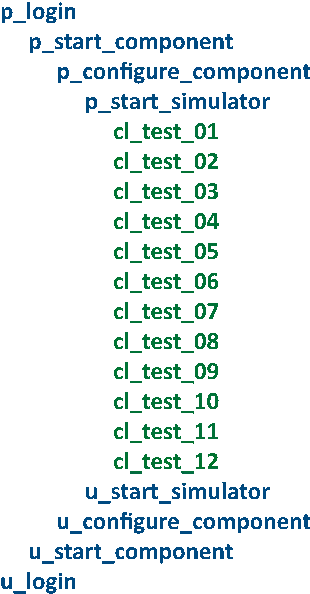
\includegraphics[scale=1]{sada_pre_optimalizaciu2}
    \caption{Príklad nevhodnej sady testov pre základný algoritmus 
             distribúcie testov}
    \label{obrazok:sada_pre_optimalizaciu2}
  \end{center}
\end{figure}



\section{Optimalizácia 3 -- distribúcia využitím podobnosti prerekvizít}
\label{sekcia:optimalizacia3}
Táto optimalizácia využíva pri distribúcií testov skutočnosť, že čím viac
skupín clusterov s~podobnými prerekvizitami existuje v~danom 
distribuovanom systéme, tým efektívnejšie vieme využiť vlastnosť 
združovania testov popísanej v~kapitole 
\ref{sekcia:princip_pouziteho_planovaca}.
Pri rozhodovaní, do ktorej z~\textit{m} skupín testov zadaných pomocou 
prepínača \textbf{-mi} vložíme aktuálnu skupinu clusterov je teda vhodné 
rozhodovať sa aj na základe tohto faktora.

Táto optimalizácia funguje tak, že sa najprv zistia všetky možné 
testovacie systémy, do ktorých je možné vložiť skupinu clusterov bez toho, 
aby sa narušilo rozloženie záťaže na týchto systémoch. 
V~prípade, že je takýchto systémov viac (čo sa v~prípade širokej škály 
clusterov s~rôznymi prerekvizitami bežne stáva),
aktuálnu skupinu clusterov automaticky nepriradíme testovaciemu systému, 
ktorý má najmenší odhadovaný čas dĺžky trvania testovania. 
Namiesto toho si pre každý takýto testovací systém spočítame počet 
prerekvizít, ktoré má spoločné s~aktuálnou skupinou clusterov, ktorú 
sa snažíme distribuovať. 

Skupinu clusterov potom priradíme do toho testovacieho systému, ktorý 
má najviac podobných prerekvizít. V~prípade, že existuje viac 
testovacích systémov, ktoré majú rovnaký počet podobných prerekvizít, 
aktuálnu skupinu testov vložíme do testovacieho systému s~najmenším 
odhadovaným časom dĺžky trvania testovania.

Počítanie podobnosti prerekvizít je jednoduchá operácia, ktorá nám vo 
výsledku zabezpečí, že sa na jednotlivých testovacích systémoch budú 
združovať clustre, ktoré majú medzi sebou podobné prerekvizity. 
Takéto clustre je potom možné efektívnejšie naplánovať a~využiť tak 
vlastnosti združovania testov.

Zapínanie tejto optimalizácie je riadené nastavením premennej 
\texttt{g\_prl\_optimize} na hodnotu väčšiu alebo rovnú 3. 
V~prípade využitia tejto optimalizácie sa zároveň aktivuje využívanie 
predošlých dvoch optimalizácií.



%
% Kapitola 6
%
\chapter{Zhodnotenie dosiahnutých výsledkov}
\label{kapitola:zhodnotenie_vysledkov}
V~nasledujúcej kapitole si porovnáme vytvorené rozšírenie plánovača s~jeho
pôvodnou verziou, ktorá nedisponovala funkcionalitou distribuovania testov.
Ukážeme si niektoré štatistiky, z~ktorých bude zrejmý prínos vytvorenia
rozšírenia pre tento nástroj. Jednotlivé štatistiky sú zbierané na základe
informácií priamo z~produktov vo firme Acision, kde sa tento plánovač testov
s~využitím distribúcie testov každodenne používa. V~kapitole si na záver 
porovnáme vplyv jednotlivých naimplementovaných optimalizácií na regresné
testovanie. 


\section{Prínos vytvorenia rozšírenia pre plánovač testov}
\label{sekcia:prinos_pouzitia}
Prínos vytvorenia rozšírenia pre distribúciu testov na viaceré testovacie 
systémy je zrejmý. Táto bakalárska práca vznikla z~potreby, že sa každodenné
regresné testovanie natiahlo na viac ako 15 hodín. Čas potrebný pre tento
typ testovania sa navyše každým pridaným testom zvyšoval. 
Za posledný rok sa v~produkte MCO zvýšil tento čas o~takmer 2 hodiny.

Z~dôvodu, že je regresné testovanie časovo náročná operácia, sa taktiež 
pri písaní nových testov bral na časovú náročnosť veľký ohľad.
V~prípade niektorých testov sa tým znížila kvalita testu, nakoľko sa tieto
testy museli obmedziť, aby nevykonávali taký veľký počet operácií.
Jednalo sa hlavne o~niektoré základné typy stress testov.

Postupom času sa musel vymyslieť spôsob, akým by bolo možné skrátiť 
dĺžku trvania regresných testov. Tým spôsobom bola distribúcia testov.

\begin{table}
  \begin{center}
    \begin{tabular}{ | p{2cm} | p{5.3cm} | p{5.3cm} | }
      \hline
      \nohyphens{počet testovacích systémov} & 
      čas potrebný pre dokončenie testovania v~produkte MCO & 
      čas potrebný pre dokončenie testovania v~produkte \nohyphens{SMSCv5} \\ \hline
      1  & 14:56:43 & 15:08:32 \\ \hline
      2  & 08:06:45 & 08:07:32 \\ \hline 
      3  & 05:32:34 & 05:36:16 \\ \hline  
      4  & 04:37:08 & 04:08:06 \\ \hline
      5  & 03:29:33 & 03:37:21 \\ \hline
      6  & 03:09:17 & 03:17:33 \\ \hline
      7  & 02:55:42 & 02:46:58 \\ \hline
      8  & 02:34:39 & 02:41:35 \\ \hline
      9  & 02:26:04 & 02:28:20 \\ \hline
      10 & 02:10:16 & 02:10:00 \\ \hline
    \end{tabular}
    \caption{Prínos použitia distribúcie testov na rôzny počet 
             testovacích systémov}
    \label{tabulka:prinos_pouzitia_distribucie}
  \end{center}
\end{table}

Tabuľka \ref{tabulka:prinos_pouzitia_distribucie} znázorňuje dĺžku trvania 
regresných testov pre produkty MCO a~SMSCv5 využitím rôznych počtov 
testovacích systémov, na ktoré je možné testy distribuovať. 
V~prípade použitia jedného testovacieho systému
je vytvorený plán testov identický s~plánom testov pred naimplementovaním 
rozšírenia pre podporu distribúcie testov. 
Údaje v~tabuľke vznikli naplánovaním regresných testov, ktoré sa 
v~spomínaných dvoch produktoch každodenne spúšťajú.
Pri plánovaní testov boli využité všetky naimplementované optimalizácie.

Z~tabuľky vyplýva, že použitím dvoch testovacích systémov skráti celkový
čas potrebný pre dokončenie testovania na približne 54\% z~celkového času 
potrebného pre dokončenie testovania v~prípade použitia jedného 
testovacieho systému.
Táto hodnota nového času testovania nie je presná polovica, nakoľko sa pri
vytváraní nových test plánov určitá množina prerekvizít spustí vždy.
Príkladom takejto prerekvizity je prerekvizita na pripojenie sa na testovací
systém, alebo na zapínanie nejakej často používanej komponenty. 

V~prípade využitia štyroch testovacích systémov efektivita distribúcie 
mierne klesá. Čas potrebný pre dokončenie testovania tvorí 
v~prípade produktu MCO približne 31\% (namiesto idálnych 25\%) 
z~času potrebného pre testovanie na jednom testovacom systéme.
V~prípade produktu SMSCv5 je táto percentuálna hodnota o~trochu 
lepšia, a~to niekde na úrovni 27\%.

Ďalším pridávaním testovacích systémov sa efektivita distribúcie 
postupne znižuje. Je to zapríčinené hlavne prekrývaním clusterov 
a~prerekvizít (hodnota test overlapping ratio použitá v~obrázku 
\ref{obrazok:ukazka_statistiky}), čo znamená že sa tieto testy spúšťajú 
vďaka distribuovaniu viacnásobne. Plánovač testov je schopný túto 
hodnotu prekrývania testov pri naplánovaní testov vypočítať.

Grafické znázornenia tabuľky \ref{tabulka:prinos_pouzitia_distribucie}
pre produkty MCO a~SMSCv5 sú umiestnené v~prílohách 
\ref{priloha:graf_mco} a~\ref{priloha:graf_smsc}.

Pre zhodnotenie prínosu vytvorenia rozšírenia plánovača testov je nutné
overiť, ako je zvládnuté rozloženie záťaže medzi jednotlivými testovacími
systémami. Pri distribuovaní testov na viaceré testovacie systémy je 
rozloženie záťaže vylepšované zbieraním štatistických informácií o~poslednom
behu testovania. 
Vo výsledku je rozloženie záťaže na jednotlivých testovacích systémoch
rovnomerné, a~pri použití niekoľkých testovacích systémoch sa 
minimálne a~maximálne zaťaženie testovacích systémov líši rádovo v~percentách.
Dôkazom toho sú napríklad nasledujúce tabuľky. 

Tabuľky \ref{tabulka:rozlozenie_zataze_mco_2} a~\ref{tabulka:rozlozenie_zataze_mco_3} 
zobrazujú rozloženie záťaže v~prípade
použitia rôzneho počtu testovacích systémov. Údaje sú zozbierané
z~distribúcie regresných testov produktu MCO. V~prípade použitia
dvoch testovacích systémov je rozdiel dĺžky testovania na týchto systémoch
prižne 17 minút. Tento čas tvorí približne 3,5\% z~maximálnej dĺžky testovania.
V~prípade použitia troch testovacích systémov je toto percento niekde 
na úrovni šiestich percent.
 
Zvyšné dve tabuľky zobrazujú rozloženie záťaže pri distribúcií testovacej
sady pre produkt SMSCv5. Tabuľka \ref{tabulka:rozlozenie_zataze_smsc_2} 
zobrazuje, že v~prípade použitia dvoch testovacích systémov je rozdiel
v~dĺžke trvania testovania približne 28 minút, čo tvorí približne 6\%
z~maximálnej dĺžky testovania. V~prípade použitia štyroch
testovacích systémov ako je zobrazených v~tabuľke \ref{tabulka:rozlozenie_zataze_smsc_4},
je rozdiel medzi najkratším a~najdlhším časom testovania približne 18 minút, čo
tvorí približne 7\% z~maximálnej dĺžky testovania.



\begin{table}[h!]
  \begin{center}
    \begin{tabular}{ | r | c | }
      \hline
      testovací systém & dĺžka testovania \\ \hline
      1  & 08:06:45  \\ \hline
      2  & 07:49:38  \\ \hline 
    \end{tabular}
    \caption{Rozloženie záťaže pre produkt MCO v~prípade použitia 2 
             testovacích systémov}
    \label{tabulka:rozlozenie_zataze_mco_2}
  \end{center}
\end{table}

\begin{table}[h!]
  \begin{center}
    \begin{tabular}{ | r | c | }
      \hline
      testovací systém & dĺžka testovania \\ \hline
      1  & 05:14:40  \\ \hline
      2  & 05:11:28  \\ \hline 
      3  & 05:32:34  \\ \hline 
    \end{tabular}
    \caption{Rozloženie záťaže pre produkt MCO v~prípade použitia 3 
             testovacích systémov}
    \label{tabulka:rozlozenie_zataze_mco_3}
  \end{center}
\end{table}


\begin{table}[h!]
  \begin{center}
    \begin{tabular}{ | r | c | }
      \hline
      testovací systém & dĺžka testovania \\ \hline
      1  & 08:07:32  \\ \hline
      2  & 07:39:21  \\ \hline 
    \end{tabular}
    \caption{Rozloženie záťaže pre produkt SMSCv5 v~prípade použitia 2 
             testovacích systémov}
    \label{tabulka:rozlozenie_zataze_smsc_2}
  \end{center}
\end{table}

\begin{table}[h!]
  \begin{center}
    \begin{tabular}{ | r | c | }
      \hline
      testovací systém & dĺžka testovania \\ \hline
      1  & 04:06:11  \\ \hline
      2  & 03:49:51  \\ \hline 
      3  & 03:58:52  \\ \hline 
      4  & 04:08:06  \\ \hline
    \end{tabular}
    \caption{Rozloženie záťaže pre produkt SMSCv5 v~prípade použitia 4 
             testovacích systémov}
    \label{tabulka:rozlozenie_zataze_smsc_4}
  \end{center}
\end{table}


\section{Porovnanie jednotlivých optimalizácií}
\label{sekcia:porovnanie_optimalizacii}
Pri porovnávaní jednotlivých optimalizácií som vychádzal z~plánovania testov
regresnej sady, ktoré sa spúšťajú denne pre dva najväčšie produkty. 
Tabuľky \ref{tabulka:porovnanie_optimalizacii_mco}
a~\ref{tabulka:porovnanie_optimalizacii_smsc} zobrazujú dĺžku trvania
regresných testov pre rôzny počet testovacích systémov a~rôzne úrovne
optimalizácie. Z~tabuliek vyplýva, že využívanie dĺžky trvania prerekvizít
a~odrekvizít ako je použité v~optimalizácií 1, nie je vždy lepšie riešenie.
Táto optimalizácia má najväčší efekt, keď sa prerekvizity spúšťajú maximálne
raz. V~prípade použitia veľkej sady testov sa však bežne niektoré prerekvizity
spúšťajú niekoľkonásobne. V~takomto prípade má optimalizácia len minimálny,
alebo dokonca aj negatívny vplyv. Optimalizácia 2 funguje na princípe rozdeľovania
veľkých skupín clusterov so spoločnými prerekvizitami. Táto optimalizácia
nadobúda efekt iba v~prípade, že je takéto skupiny nutné rozdeliť aby sme 
zachovali optimálne rozloženie záťaže. V~prípade regresných testov sa však 
takéto veľké skupiny testov dokážu distribuovať aj bez toho, aby to narušilo
rozloženie záťaže. Znova teda platí, že táto optimalizácia má efekt skôr na
menší počet testov. 

Z~pohľadu regresného testovania má však veľký vplyv posledná optimalizácia.
Táto optimalizácia sa snaží distribuovať clustre na testovacie systémy tak,
aby sa na každom testovacom systéme združovali clustre s~podobnými prerekvizitami.
Je to z~dôvodu, aby plánovač testov mohol využiť svoju vlastnosť združovania
testov. Z~tabuliek vyplýva, že tento typ optimalizácie je schopný skrátiť
čas potrebný na dokončenie regresného testovania aj o~niekoľko desiatok minút.


\begin{table}
  \begin{center}
    \begin{tabular}{ | C{2.9cm} | C{2.8cm} | C{2.51cm} | C{2.51cm} | C{2.51cm} | }
      \hline
      & \multicolumn{4}{c|}{Dĺžka regresného testovania} \\ \cline{2-5}
      počet testovacích systémov & bez optimalizácií & optimalizácia 1 & optimalizácia 2 & optimalizácia 3 \\ \hline
      1  & 14:56:43 & 14:56:43 & 14:56:43 & 14:56:43 \\ \hline
      2  & 08:53:16 & 08:40:17 & 08:40:17 & 08:06:45 \\ \hline
      3  & 06:19:57 & 06:22:37 & 06:22:37 & 05:32:34 \\ \hline
      4  & 05:03:54 & 05:05:24 & 05:05:24 & 04:37:08 \\ \hline
      5  & 04:13:29 & 04:15:41 & 04:15:41 & 03:29:33 \\ \hline
      6  & 03:37:58 & 03:40:10 & 03:40:10 & 03:09:17 \\ \hline
      7  & 03:12:31 & 03:26:33 & 03:26:33 & 02:55:42 \\ \hline
      8  & 03:00:58 & 02:52:57 & 02:52:57 & 02:34:39 \\ \hline
      9  & 02:45:07 & 02:35:39 & 02:35:39 & 02:26:04 \\ \hline
      10 & 02:40:52 & 02:41:40 & 02:41:40 & 02:10:16 \\ \hline
    \end{tabular}
    \caption{Porovnanie jednotlivých optimalizácií pri plánovaní regresných testov v~produkte MCO}
    \label{tabulka:porovnanie_optimalizacii_mco}
  \end{center}
\end{table}

\begin{table}
  \begin{center}
    \begin{tabular}{ | R{2.9cm} | C{2.8cm} | C{2.51cm} | C{2.51cm} | C{2.51cm} | }
      \hline
      & \multicolumn{4}{c|}{Dĺžka regresného testovania} \\ \cline{2-5}
      počet testovacích systémov & bez optimalizácií & optimalizácia 1 & optimalizácia 2 & optimalizácia 3 \\ \hline
      1  & 15:08:32 & 15:08:32 & 15:08:32 & 15:08:32 \\ \hline
      2  & 08:19:32 & 08:23:25 & 08:23:25 & 08:07:32 \\ \hline
      3  & 05:54:31 & 05:53:21 & 05:53:21 & 05:36:16 \\ \hline
      4  & 04:40:18 & 04:51:22 & 04:51:22 & 04:08:06 \\ \hline
      5  & 03:52:44 & 03:50:06 & 03:50:06 & 03:37:21 \\ \hline
      6  & 03:15:13 & 03:18:23 & 03:18:23 & 03:17:33 \\ \hline
      7  & 02:53:37 & 03:00:35 & 03:00:35 & 02:46:58 \\ \hline
      8  & 02:38:00 & 02:46:31 & 02:46:31 & 02:41:35 \\ \hline
      9  & 02:27:12 & 02:27:25 & 02:27:25 & 02:28:20 \\ \hline
      10 & 02:21:39 & 02:08:54 & 02:08:54 & 02:10:00 \\ \hline
    \end{tabular}
    \caption{Porovnanie jednotlivých optimalizácií pri plánovaní regresných testov v~produkte SMSCv5}
    \label{tabulka:porovnanie_optimalizacii_smsc}
  \end{center}
\end{table}

Pre demonštrovanie optimalizácie 2 si uvedieme naplánovanie funkcionality
\textit{addrtran} pre produkt MCO. Táto funkcionalita pozostáva z~niekoľko
desiatok testov, z~ktorých väčšina má rovnakú množinu prerekvizít. 
Testy v~tejto funkcionalite majú len 2 množiny prerekvizít, takže všetky
clustre sa rozdelia len do dvoch skupín testov. 
Tabuľka \ref{tabulka:porovnanie_optimalizacie_2} zobrazuje dĺžky trvania
testovania tejto funkcionality a~efekt spomínanej optimalizácie. 
Pri plánovaní tejto funkcionality bol využitý parameter \textit{-wp}, 
ktorý zapríčiní, že sa funkcionalita naplánuje bez použitia Preoptov.

\begin{table}[h!]
  \begin{center}
    \begin{tabular}{ | C{1.5cm} | C{4cm} | C{4.5cm} | }
      \hline
      testovací systém & dĺžka testovania bez využitia optimalizácie & dĺžka testovania s~využitím optimalizácie \\ \hline
      1 & 11:31 &  11:31 \\ \hline \hline
      1 & 03:46 &  07:27 \\ \hline 
      2 & 10:54 &  07:52 \\ \hline \hline
      1 & 03:46 &  06:00 \\ \hline
      2 & 10:54 &  06:32 \\ \hline
      3 &   -   &  06:35 \\ \hline \hline
      1 & 03:46 &  05:35 \\ \hline
      2 & 10:54 &  05:34 \\ \hline
      3 &   -   &  05:52 \\ \hline 
      4 &   -   &  05:54 \\ \hline \hline
      1 & 03:46 &  05:14 \\ \hline
      2 & 10:54 &  05:02 \\ \hline
      3 &   -   &  05:28 \\ \hline
      4 &   -   &  05:29 \\ \hline
      5 &   -   &  05:30 \\ \hline
    \end{tabular}
    \caption{Porovnanie vplyvu optimalizácie 2 na jednotlivé testovacie
             systémy}
    \label{tabulka:porovnanie_optimalizacie_2}
  \end{center}
\end{table}

Z~tabuľky vyplýva, že v~prípade nevyužitia optimalizácie sme schopní distribuovať 
iba skupiny clusterov s~rovnakými prerekvizitami. Nakoľko máme takéto skupiny 
iba dve, sme schopní využiť iba dva testovacie systémy. V~prípade využitia
optimalizácie sme schopní rozdelovať skupiny clusterov na menšie a~využiť 
tým viac testovacích systémov. V~prípade využitia dvoch testovacích systémov
je vidieť efektivitu tejto optimalizácie, nakoľko sa dve skupiny clusterov
rozdelia tak, aby sa dva testovacie systémy využili rovnomerne. 
Odhadovaný čas testovania sa na týchto dvoch systémoch bude líšiť o~25 sekúnd,
namiesto takmer siedmych minút, o~ktoré by sa tento čas líšil v~prípade nevyužitia
optimalizácie. 

V~prípade použitia viacerých testovacích systémov môžeme na tabuľke jasne vidieť,
že sa niektoré testovacie systémy bez použitia optimalizácie nevyužijú. 
V~prípade využitia optimalizácie sa skupiny clusterov rozdelia tak efektívne,
že rozdiely dĺžky trvania testovania medzi jednotlivými testovacími systémami 
sú rádovo v~sekundách.


%
% Kapitola 7
%
\chapter{Záver}
\label{kapitola:zaver}

\section{Zhrnutie}
\label{sekcia:zhrnutie}

\section{Možnosti ďalšieho vývoja}
\label{sekcia:moznosti_dalsieho_vyvoja}
%=========================================================================
